% !TeX root = RJwrapper.tex
\title{Admix: An R Package for Estimation, Test and Clustering in Admixture Models}


\author{by Xavier Milhaud, Denys Pommeret, Yahia Salhi, and Pierre Vandekerkhove}

\maketitle

\abstract{%
The R package admix, available on CRAN, implements a wide variety of functions dedicated to estimation, tests and clustering of admixture models, also known as contamination models. Such models are two-component mixture distributions having only one single known component. They are particularly useful when a known random phenomenon is contaminated by an unknown/unexpected random effect. We propose in this setup to estimate semiparametrically the unknown quantities of the model, and compare or cluster the unknown sources of randomness across different samples without making any parametric assumptions about them. The admix package appears thus as a powerful tool for applications where latent variables induce hidden heterogeneity, often revealed through multimodality in data distributions.
}

\section{Introduction}\label{introduction}

The general framework is the semiparametric two-component mixture model, with cumulative distribution function (cdf)
\begin{equation}
 L(x) = (1-p)G(x)+pF(x), \quad x \in \mathbb{R},
 \label{eq:model}
\end{equation}
where \(G\) is a known cdf and where the unknown parameters are the mixture proportion \(p\in ]0,1[\) and the cdf \(F\) which is not supposed to belong to any parametric family. The above model \eqref{eq:model}, so-called \strong{contamination} or \strong{admixture} model, has been widely investigated in the last decades, see for instance \citet{Bordes+Vandekerkhove:2010}, \citet{Cai+Jin:2010} or \citet{Celisse+Robin:2010} among others. Such a modelling arises in various applications, in particular during crisis times where some populations are impacted when others are not concerned yet. In genomics, studying the genetic make-up of populations has been the subject of extensive attention. The admixture behaviour is of paramount importance in comparing the populations with known ancestors and exhibits linkage relationships between them \citep{Loh+Lipson+Patterson+Moorjani+Pickrell+Reich+Berger:2013}.

As an illustration, \citet{McLachlan+Bean+Jones:2006} proposed a method for detecting differentially expressed genes in breast cancer tissues, from women carrying hereditary BRCA1 or BRCA2 mutations \citep{Hedenfalk+Duggan+Chen:2001}. Their approach is based on a two-component mixture model with one known component. More specifically, a \(z\)-score type statistic is built for each gene, distributed according to a mixture model where the gene is either normally expressed or not. When it is normally expressed, its \(z\)-score is expected to follow a (known) standard Gaussian distribution. Otherwise, the \(z\)-score is modeled by a trash (unknown) distribution. Figure \ref{fig:Figure1-latex} shows the histogram of the 3,170 observed \(z\)-scores, along with its decomposition into two density components. Parameter estimation in \citet{Pommeret+Vandekerkhove:2019} resulted in a proportion \(p=0.65\) for the known \(\mathcal{N}(0,1)\) component, while the second component follows a Gaussian distribution with mean 1.5 and variance 0.98. In this context, it may be useful to identify the gene family of not normally expressed genes, and then classify them by gene family type. This is one illustration of what the admix package allows one to do.

\begin{figure}

{\centering 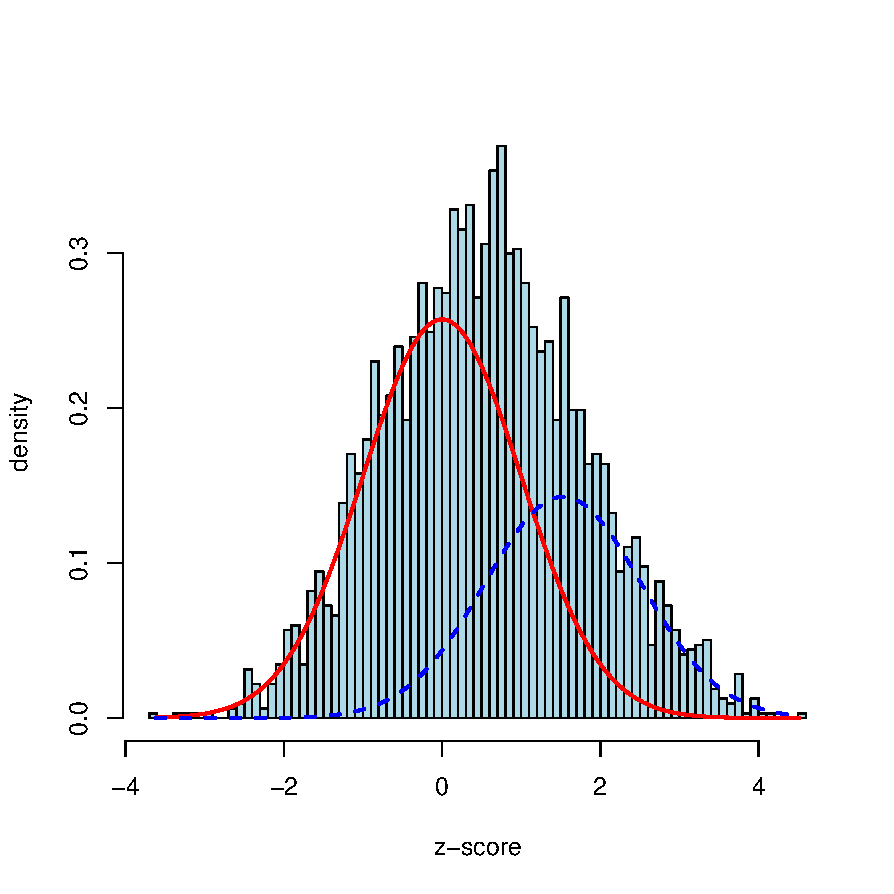
\includegraphics[width=0.55\linewidth,height=0.27\textheight]{FigureIntroZ} 

}

\caption{Histogram of $z$-scores in the breast cancer study, where the known component (in red) is $\mathcal{N}(0,1)$, and the unknown one is estimated as $\mathcal{N}(1.5,0.98)$ with proportion $p=0.35$.}\label{fig:Figure1-latex}
\end{figure}

More generally, such a problem arises when a known random phenomenon is contaminated by an unknown random effect. The interest in such models is twofold: i) understand how and to which extent the original population distribution \(G\) has been contaminated or distorted by the extra component distribution \(F\), ii) compare this impact over various populations. In that latter case, the data of interest is hence made of \(K\) independent and identically distributed (i.i.d.) samples
\(X_1=(X_{1,1},\dots,X_{1,n_1}),\dots, X_K=(X_{K,1},\dots, X_{K,n_K})\) with cdfs:
\begin{equation}
        L_i(x) = (1-p_i) \, G_i(x) + p_i \, F_i(x), \quad x \in  \mathbb{R}, \quad i=1,\dots, K,
        \label{eq:models}
\end{equation}
where \(p_1,\dots, p_K\) are the unknown mixture proportions and \(F_1, \dots, F_K\) are unknown cdf components.
Hereafter, we consider situations where the \(G_i\)'s and \(F_i\)'s distributions are: (i) absolutely continuous with respect to the Lebesgue measure, supported over \(\mathbb{R}\), \(\mathbb{R}^+\) or intervals of \(\mathbb{R}\); (ii) finite discrete or \(\mathbb{N}\)-discrete distributions such as Binomial or Poisson; (iii) a mixture of a discrete and an absolutely continuous distribution.
All our implementations still work in such frameworks.

The goal of the package \CRANpkg{admix} is to provide consistent numerical solutions for the following tasks:

\begin{itemize}
\tightlist
\item
  Provide robust estimations of the unknown parameters, \emph{i.e.} \((p_i,F_i)\) for \(i=1,\dots,K\);
\item
  Test the equality of the \(F_i\)'s involved in a sub-\(k\)-sample for \(2 \leq k \leq K\);
\item
  Detect potential clusters (samples sharing the same unknown cdf) inside the \(K\)-sample.
\end{itemize}

As might be expected given recent advances, and contrary to the parametric mixture model framework, there are very few implementations dealing with semiparametric mixture models. As far as we are aware, the \CRANpkg{admix} package is the first to deal with admixture models in such a general setting, followed by the packages \CRANpkg{MixSemiRob} \citep{Kang+Shen+Yao+Xiang+Ge:2023} and \pkg{mixmodel}\footnote{Not on CRAN, but available at \url{https://github.com/rohitpatra/mixmodel}.} \citep{Patra+Sen:2016}. Other recent packages are \CRANpkg{admixr} \citep{Petr:2020} and \pkg{admixturegraph} \citep{Leppala+Nielsen+Mailund:2017}, but they are only targeted towards genomic studies and strongly connected to \pkg{ADMIXTOOLS 2}\footnote{For further information, see \url{https://uqrmaie1.github.io/admixtools/index.html}.}. We also mention \CRANpkg{mclust} \citep{Scrucca+Fraley+Murphy+Raftery:2023} and \CRANpkg{ContaminatedMixt} \citep{Punzo+Mazza+McNicholas:2018}, despite they focus on model-based clustering and classification relying on Gaussian mixtures only. More generally, numerous R packages dealing with mixture distributions have already been proposed, see for instance the most famous of them, \CRANpkg{mixtools} \citep{Benaglia+Chauveau+Hunter+Young:2009}. The CRAN Task View \ctv{Cluster Analysis and Finite Mixture Models} provides a more exhaustive list of them. However, these packages mostly rely on parametric assumptions made on the mixture component distributions, which is too restrictive in the context of admixture models where no knowledge about the contamination effect is \emph{a priori} accessible. This brief review highlights the need to develop new tools in this area.

The rest of the paper is organized as follows. Section \ref{sec:methodo} describes the theoretical properties of the estimation and testing strategies implemented in our package. Section \ref{sec:overview} gives a synthetic overview of the package, focusing on core functions and their structure. Then, Section \ref{sec:practicalUse} provides some examples on how to use the package in practice.

\section{Theory of implemented statistical methodologies}\label{sec:methodo}

The \CRANpkg{admix} package \citep{admix:2025} provides several ways to perform estimation and tests in admixture models, all of them coming from publications in high-ranking statistical journals. Hereafter, we review the main ideas on which the package is grounded. We present first the different estimation methods available, and talk about associated testing strategies. Finally, we discuss the clustering scheme that has been proposed in the specific \(K\)-sample setup to create groups of samples similarly contaminated. To be self-contained, the paper provides models, assumptions and key ideas underlying each method. However, for the sake of conciseness, we briefly detail and comment these methods. The reader can find further details, especially about identifiability and consistency, in the cited references.

\subsection{Estimation of the mixture proportion}\label{sec:estimTechniques}

Inside the available \(K\) samples, let us consider \(X_i=(X_{i,1}, \dots, X_{i,n_i})\) the \(i\)-th sample, for \(i=1,\dots,K\), made of \(n_i\) independent and identically distributed random variables with common cdf \(L_i\):
\begin{equation}
  L_i(x) = (1-p_i) \, G_i(x) + p_i \, F_i(x), \qquad x \in \mathbb{R},
\label{eq:ithAdmixture}
\end{equation}
where \(G_i\) is a known cdf when the mixture proportion \(p_i\) and the extra cdf \(F_i\) are unknown.

The estimation step first seeks a robust estimation of \(p_i\), followed by an estimation of \(F_i\) based on plugged-in inversion formula involving the previous \(p_i\) estimation and the empirical cdf of the dataset \(X_i\). In the sequel, we denote respectively by \(\ell_i\), \(f_i\) and \(g_i\) the probability density function (pdf) associated with \(L_i\), \(F_i\) and \(G_i\). Three estimation procedures of \(p_i\) can be used:

\begin{itemize}
\item
  The \emph{PS} estimator \citep{Patra+Sen:2016}, which works under tail conditions about \(F_i\) and \(G_i\), and does not require any specific shape constraint thanks to a relevant definition of identifiability in the case of semiparametric admixture models. This method provides a consistent estimator of \(p_i\), which fails to be asymptotically normal \citep[see Theorem 4 in][]{Patra+Sen:2016}.
\item
  The \emph{BVdk} estimator \citep{Bordes+Delmas+Vandekerkhove:2006} satisfies a joint functional central limit theorem \citep[see also][]{Bordes+Vandekerkhove:2010}, in the context where \(f_i\) and \(g_i\) are supposed to be symmetric densities with respect to some location parameters. The procedure provides \(\sqrt{n}\)-consistent estimators of both \(p_i\) and the location parameter, along with the unknown cdf.
\item
  The \emph{IBM} estimator \citep{Milhaud+Pommeret+Salhi+Vandekerkhove:2023}, developed in a testing perspective, provides \(\sqrt{n}\)-consistent estimators in the two-sample case when the unknown components in both samples share the same distribution (null hypothesis). When this condition is not satisfied, the asymptotic behavior of the IBM estimator along with the associated test statistic is also explicitly derived.
\end{itemize}

\subsubsection{The PS estimator}\label{the-ps-estimator}

In contrast with previous works about semiparametric mixture estimation, see \citet{Bordes+Mottelet+Vandekerkhove:2006}, \citet{Bordes+Delmas+Vandekerkhove:2006} or \citet{Butucea+Tzoumpe+Vandekerkhove:2017}, all based on symmetry type assumption about the unknown component, \citet{Patra+Sen:2016} proposed to relax this restrictive shape constraint by noticing that model \eqref{eq:ithAdmixture} could also be rewritten as
\[L_i(x) = (1-[p_i+\lambda]) G_i(x) + [p_i+\lambda] \left( \dfrac{p_i}{p_i+\lambda} F_i(x) + \dfrac{\lambda}{p_i+\lambda} G_i(x) \right), \qquad x \in \mathbb{R},\]
with \(0 \leq \lambda \leq 1-p_i\), and where \((p_i F_i(x) + \lambda G_i(x))/(p_i+\lambda)\) could be thought as the nonparametric component (denote further \(\pi_i = p_i+\lambda\)). This writing shows a clear lack of identifiability since \(p_i\) is not uniquely defined. The authors propose to solve this lack of identifiability by considering the following definition of the \emph{correct} parameter
\begin{equation}
p_{0,i} := \inf \left\{ \pi_i \in (0,1] \, : \, \frac{L_i - (1-\pi_i)G_i}{\pi_i} \; \text{is a true cdf} \right\},
\label{eq:correctprop}
\end{equation}
and estimate this parameter by
\[
\hat p_i^{c_n} = \inf \left\{ \pi_i \in (0,1) \, : \, 
\pi_i d_n\!\left( F_i(\cdot,\pi_i,\hat L_{i,n}), \check{F}_{i,n}(\cdot,\pi_i)\right) 
\leq \frac{c_n}{\sqrt{n_i}} \right\},
\]
where the tuning parameter \(c_n \to +\infty\) not too fast, \(d_n\) is the empirical \(L^2(\mathbb L_{i,n})\) distance,
\(\check F_{i,n}(\cdot,\pi_i)\) is the closest cdf from \(F_i(\cdot,\pi_i,\hat L_{i,n})\) in the \(L^2(\mathbb L_{i,n})\) sense obtained by isotonic regression and the pool-adjacent-violators algorithm. The authors prove the consistency of the estimator \(\hat p_i^{c_n}\) and provide its convergence rate \citep[see Theorem 4 in][]{Patra+Sen:2016}. However, there is no central limit theorem for this estimator, and cross-validations are often required to improve the estimation of the unknown correct mixture proportion \(p_{0,i}\) defined in \eqref{eq:correctprop}.

\subsubsection{The BVdk estimator}\label{the-bvdk-estimator}

As already mentioned, the \emph{BVdk} estimator relies on a symmetry assumption regarding the unknown component \(F_i\) about some location parameter \(\mu_i\), see \citeauthor{Bordes+Vandekerkhove:2010} \citetext{\citeyear{Bordes+Vandekerkhove:2010}; \citealp[and previous works by][]{Bordes+Delmas+Vandekerkhove:2006}}. Suppose that we observe an i.i.d. sample \(X_i=(X_{i,1}, \dots, X_{i,n_i})\) with cdf \(L_i\) defined by
\begin{equation}
  L_i(x) = (1-p_i) \, G_i(x) + p_i \, F_i(x - \mu_i), \qquad x \in \mathbb{R},
\label{eq:symmetricUnknownComp}
\end{equation}
where the unknown Euclidean parameters to be estimated are \(p_i\in ]0,1[\) and \(\mu_i\in \mathbb{R}\). Under some identifiability assumptions, the following inversion formula with parameters \((p_i,\mu_i)\) holds:
\[
F_i(x) = \frac{1}{p_i} \left( L_i(x+\mu_i) - (1-p_i) G_i(x+\mu_i) \right), \qquad x \in \mathbb{R}.
\]
In addition, according to the symmetry assumption, one knows that \(F_i(x) = 1 - F_i(-x)\) for all \(x \in \mathbb{R}\). Keeping this in mind, we can introduce the two following functions
\[
H_1(x; p_i,\mu_i, L_i) = \frac{1}{p_i} L_i(x+\mu_i) - \frac{1-p_i}{p_i} G_i(x+\mu_i),
\]
and
\[
H_2(x; p_i,\mu_i, L_i) = 1 - \frac{1}{p_i} L_i(-x+\mu_i) + \frac{1-p_i}{p_i} G_i(-x+\mu_i).
\]
Using the symmetry of \(F_i\) and denoting \((p_0, \mu_0)\) the true (unknown) Euclidean parameters, we have
\[
H(x; p_{0,i}, \mu_{0,i}, L_i) = H_1(x; p_{0,i},\mu_{0,i}, L_i) - H_2(x; p_{0,i},\mu_{0,i}, L_i) = 0, \qquad \mbox{for all } x \in \mathbb{R}.
\]

In this setup, one expects that for all \((p_i,\mu_i) \neq (p_{0,i},\mu_{0,i})\) an \emph{ad hoc} \(\mathbb{R}\)-weighted quadratic norm applied to the function \(H\) will be strictly positive. This leads to consider the \emph{discrepancy measure}, also called \emph{contrast function}, given by
\[
d(p_i,\mu_i) = \int_{\mathbb{R}} H^2(x; p_i,\mu_i, L_i) \, dL_i(x).
\]
The final step consists then in estimating the Euclidean parameters, based on an adequate empirical version \(d_{n_i}\) of the contrast function \(d\), as follows:
\begin{equation}
  (\hat{p}_{i},\hat{\mu}_{i}) = \arg\min_{(p_i,\mu_i)\in \Theta} d_{n_i}(p_i,\mu_i),
  \, \text{where} \,
  d_{n_i}(p_i,\mu_i) = \int_{\mathbb{R}} H^2(x; p_i,\mu_i, \tilde L_i) \, d\hat L_i(x),
\label{eq:contrastEmpBVdk}
\end{equation}
where \(\hat L_i\) and \(\tilde L_i\) denote respectively the empirical and the kernel-smoothed version of the cdf \(L_i\) and \(\Theta\) is a compact set of \(]0,1[\times \mathbb R\). Identifiability along with kernel conditions are established in \citet{Bordes+Vandekerkhove:2010} to prove the asymptotic normality of the vector \((\hat{\mu}_{i},\hat{p}_{i},\hat{F}_{i}(\cdot))\), see Theorem 3.2 of the paper. The authors also show how to estimate consistently the variance-covariance matrix involved in their functional central limit theorem. This matrix is key to get a correct insight about the accuracy of the obtained estimates, and fundamental for future derivation of statistical tests.

\subsubsection{The IBM estimator}\label{the-ibm-estimator}

Consider the two-sample case involving two separate i.i.d. samples \(X_i=(X_{i,l})_{1 \leq l \leq n_i}\) and \(X_j=(X_{j,l})_{1 \leq l \leq n_j}\) distributed respectively according to the contamination model \eqref{eq:ithAdmixture}. Under the assumption \(H_0: ~F_i=F_j\), \citet{Milhaud+Pommeret+Salhi+Vandekerkhove:2023} propose, under very minimal conditions, a method to \(\sqrt{n}\)-consistently estimate, with a fully derived functional central limit theorem, the proportion parameters \(p_i\) and \(p_j\), along with the unknown cdf (\(F_i=F_j\)). The idea is to get benefit from the two separate samples at disposal (sharing the same unknown component under \(H_0\)) to test whether the equality of their unknown contaminating distributions \(F_i\) and \(F_j\) is plausible or not. To get their theoretical result, the authors first consider an inversion step which allows them to define two parametric function families \(\mathcal{F}_k\) (\(k=i,j\)) such that
\begin{equation}
  \mathcal{F}_k = \{ F_k(x,p_k) := (L_k(x) - (1-p_k)G_k(x))/p_k, \; p_k \in \Theta_k, \; x \in \mathbb{R} \},
\label{eq:paramFamily}
\end{equation}
with \(\Theta_k = [\delta_{1,k},\delta_{2,k}]\) where \(0 < \delta_{1,k} < 1 < \delta_{2,k} < +\infty\).

They propose to call \emph{IBM-method} the semiparametric estimation strategy based on this `Inversion' step followed by the `Best Matching' step between the \(\mathcal{F}_i\) and \(\mathcal{F}_j\) families, to look at how close they can possibly be. In this view, they introduce the best-matching step by considering the discrepancy measure
\begin{equation}
  d(\theta) = \int_{\mathbb{R}} \big(F_i(x,p_i) - F_j(x,p_j)\big)^2 \, dU(x),
\label{eq:equationd}
\end{equation}
where \(\theta=(p_i,p_j) \in \Theta_i\times \Theta_j\), \(U\) is a finite integrating measure over \(\mathbb R\) that allows one to weigh more or less some domains of the observed distribution (in practice \(U\) is a Uniform distribution over the observations support). The best matching is reached when \(d(\theta) = 0\), which condition is achieved if and only if \(\theta=\theta_0=(p_{0,i},p_{0,j})\) the true value of the parameter under identifiability conditions, see condition (I) in Section 3 of \citet{Milhaud+Pommeret+Salhi+Vandekerkhove:2023}.

The final step consists then in estimating the Euclidean parameters, based on an adequate empirical version \(d_{n_i,n_j}\) of the contrast function \(d\), as follows:
\begin{equation}
  (\hat{p}_{i}, \hat{p}_{j}) = \arg\min_{(p_i,p_j)\in \Theta} d_{n_i,n_j}(p_i,p_j),
\label{eq:contratEmpIBM}
\end{equation}
where
\[
  \hat d_{n_i,n_j}(p_i,p_j) = \int_{\mathbb{R}} \big(\tilde F_i(x,p_i) - \tilde F_j(x,p_j)\big)^2 \, dU(x),
\]
and \(\tilde F_i\) (respectively \(\tilde F_j\)) belongs to the parametric family defined in \eqref{eq:paramFamily} (replacing \(L_i\) by its empirical estimator \(\hat{L}_i\)). The asymptotic properties of the above estimator are detailed under \(H_0\) and \(H_1\) in \citet{Milhaud+Pommeret+Salhi+Vandekerkhove:2023}, see Theorems 1-2.

\subsection{Estimation of the decontaminated cumulative distribution function}\label{sec:decontamine}

Once the weight \(p_i\) of the unknown component distribution \(F_i\) has been consistently estimated, it is pretty straightforward to estimate the unknown cdf \(F_i\) itself by using the inversion formula\\
\begin{equation}
  \hat{F}_i(x) = \frac{\hat{L}_i(x) - (1-\hat{p}_i)G_i(x)}{\hat{p}_i},
\label{eq:decontaminatedCDF}
\end{equation}
where the estimators \(\hat{L}_i\) and \(\hat{p}_i\) respectively stand for the empirical cumulative distribution function of the observations and the estimated mixture proportion. The estimator \(\hat{F}_i(x)\) is the so-called \emph{decontaminated} version of the unknown cdf of the admixture model.

\subsection{Testing strategies}\label{sec:testingMeth}

Consider \(K\) separate admixture samples drawn from \eqref{eq:ithAdmixture}. Two questions then naturally arise:

\emph{i)} Do the \(F_i\)'s belong to one given parametric family?

\emph{ii)} Are some \(F_i\)'s, involved in the \(K\)-sample, possibly the same?

In the sequel, these two questions will be simply referred to as the \emph{i)} and \emph{ii)} testing problem. We now introduce the methods we implemented in the \CRANpkg{admix} package to answer these questions.

\subsubsection{Polynomial expansions (1-sample and 2-sample cases)}\label{polynomial-expansions-1-sample-and-2-sample-cases}

In \citet{Pommeret+Vandekerkhove:2019}, the authors consider admixture models in the 1-sample case having a probability density function (pdf) with respect to the Lebesgue measure:
\begin{equation}
  \ell_i(x) = (1-p) g_i(x) + p f_i(x),\quad x\in \mathbb{R},
\label{eq:admixDensite}
\end{equation}
and are interested in testing if the unknown pdf \(f_i\), associated with \(F_i\) in model \eqref{eq:ithAdmixture}, belongs to a given parametric family (in practice \(i=1\) since there is only one sample available). The hypotheses of the test, answering the above \emph{i)} testing problem in the absolutely continuous case, are expressed as follows:
\begin{equation}
  H_0 : f_i \in {\mathcal F} = \{ f_{\xi} ;  \xi \in \Lambda \} \quad \text{against} \quad H_1 : f_i \notin {\mathcal F},
\label{eq:Hsimple}
\end{equation}
where \(f_{\xi}\) is a pdf parametrized by an Euclidean parameter \(\xi\) belonging to a parametric space \(\Lambda\). The authors focus on the so-called \emph{Gaussianity test}, meaning that \(f_i\) is tested to be a Gaussian density.
The main idea is to use the expansions of the densities \(\ell_i\), \(f_i\), and \(g_i\) in a dense basis \(\{ Q_r ; r \in \mathbb N \}\) (e.g.~the Hermite polynomials in the Gaussian case), assuming that \(\ell_i\) is square integrable:
\begin{equation}
  f_i(x) =  \displaystyle\sum_{r\in\mathbb N} a_r Q_r(x).
\label{eq:ortho-admixtureDensity}
\end{equation}
The test statistics have the form
\[
  T_{R} = \sum_{r \leq R} \frac{(\widehat a_r - a_r(\widehat \xi))^2}{\widehat{\mathrm{Var}}(\widehat a_r - a_r(\widehat \xi))},
\]
which compare pairwise the \(a_r\)'s coefficients estimated under a relaxed set of conditions versus under the \(H_0\) assumption, \emph{i.e.} where each \(\widehat a_r\) is an empirical estimator of \(a_r\) obtained using the inversion formula \eqref{eq:decontaminatedCDF}, and \(a_r(\widehat \xi)\) is the estimated coefficient under the null \(H_0\) based on the \emph{PS} or \emph{BVdk} estimator.
Theoretical guarantees of this testing strategy remain valid if the plugged estimators are \(\sqrt{n}\)-consistent, which is not the case with the \emph{PS} estimator. However, in practice and from our experiments, both estimators provide satisfactory results in terms of test efficiency.

A penalized rule is used to select the number \(R\) of components to be integrated into the test statistic. Theoretically it is assumed that \(R\) is lower than \(R_n=o(\log(n))\), but in practice \(R_n\) is set to 3 by default (which can easily be modified by the user through arguments inside the appropriate function) as this value seems to provide satisfactory results in a wide range of situations. Writing
\[
S_n = \min \left( \arg\max_{1 \leq R \leq R_n} \big( n^{\lambda-1} T_R - R \log(n) \big) \right),
\]
with \(0 < \lambda < 1/2\),
\citet{Pommeret+Vandekerkhove:2019} show that under the null \(H_0\) the penalized test statistic \(T_{S_n}\) tends to a chi-square distribution with one degree of freedom, denoted further \(\chi^2_1\), see Theorem 2 and Corollary 3 in \citet{Pommeret+Vandekerkhove:2019}.

An extension of this test to the 2-sample case, considered as a first brick to answer the above \emph{ii)} testing problem, has been proposed later in \citet{Milhaud+Pommeret+Salhi+Vandekerkhove:2022}. In their paper, the authors develop a testing methodology suited for the comparison of two symmetric unknown component densities \(f_i\) and \(f_j\) (\(i \neq j, \; 1 \leq i,j \leq K\)), in line with the hypothesis testing problem
\begin{equation}
  H_0: F_i=F_j  \quad \text{against} \quad  F_i \neq F_j.
\label{eq:twoSample-test}
\end{equation}

Here, \(i\) and \(j\) represent any pair of populations among the \(K\) samples. As in the 1-sample case, they propose a semiparametric penalized \(\chi^2\)-type testing procedure allowing a pairwise comparison of the unknown components. The test procedure consists in expanding the two unknown densities \(f_i\) and \(f_j\) in an orthogonal polynomial basis, and then comparing, with an ad hoc method, their coefficients up to a parsimonious rank \(R\) selected according to a data-driven technique.

Basically, denoting \(\mathcal{Q} = \{Q_r; \, r \in \mathbb{N}\}\) an orthonormal basis of the \(L^2(\nu)\) space, where \(\nu\) is a common reference measure for the densities expressed in \eqref{eq:admixDensite}, the densities of the model can be rewritten as
\begin{equation}
  \ell_k(x) = \sum_{r \geq 0} \ell_{k,r} Q_r(x), \quad 
  \text{with } \ell_{k,r} = \int_{\mathbb{R}} Q_r(x) \ell_k(x) \, \nu(dx), \quad k=i,j.
\label{eq:densityDecomp}
\end{equation}

The densities \(f_k\) and \(g_k\) (\(k=i,j\)) can be decomposed in the same way, and from \eqref{eq:ithAdmixture} and \eqref{eq:densityDecomp}, we deduce that
\[\ell_{k,r} = p_k \, f_{k,r} + (1-p_k) \, g_{k,r}.\]
Finally, testing \(H_0: \, f_i = f_j\) in this set-up is equivalent to the following statistical test:
\begin{equation}
  H_0: \; a_{i,r} \; = \;  a_{j,r}, \quad r=1,2, \dots,
\label{eq:newTestOrtho}
\end{equation}
where
\begin{equation}
  a_{k,r} = \frac{\ell_{k,r} - (1-p_k) g_{k,r}}{p_k}, \quad k=i,j.
\label{eq:coeffs}
\end{equation}

Given that \(g_i\) and \(g_j\) are fully known densities (and that their respective coefficients \(g_{i,r}\) and \(g_{j,r}\) in the polynomial basis expansions are therefore exactly known), it remains to estimate the expansion coefficients of \(\ell_i\), \(\ell_j\) along with unknown proportions \(p_i\) and \(p_j\) in \eqref{eq:coeffs}. To build the test statistic, the idea is then to explore pairwise the difference of such coefficients up to some order \(R_n\), and incorporate these differences into a test statistic. Similarly to \citet{Pommeret+Vandekerkhove:2019}, the test statistics have the following expression
\[
T_{R} = \sum_{r \leq R} \frac{(\widehat a_{i,r} - \widehat a_{j,r})^2}{\widehat{\mathrm{Var}}(\widehat a_{i,r} - \widehat a_{j,r})},
\]
where each \(\widehat a_{i,r}\) is an estimator of \(a_{i,r}\) obtained by combining empirical estimators with the estimators of \(p_i\).
A penalized rule is used to select the number of components \(S_{n_i,n_j}\) in the test statistic:
\[
S_{n_i,n_j} = \min \Biggl( \arg\max_{1 \leq R \leq R_n} \left( \Bigl(\frac{n_i n_j}{n_i+n_j}\Bigr)^{\lambda - 1} T_R - R \log\Bigl(\frac{n_i n_j}{n_i+n_j}\Bigr) \right) \Biggr),
\]
with \(0 < \lambda < 1/2\).

To get valid asymptotic results, it is assumed that \(R_n=o(\log(n_i n_j/(n_i+n_j)))\). The parameter \(\lambda\) can be fixed arbitrarily close to 0.5 to increase the power of the test, or close to 0 to get a more conservative test. Under the null hypothesis, \citet{Milhaud+Pommeret+Salhi+Vandekerkhove:2022} prove that the penalized test statistic \(T_{S_{n_i,n_j}}\) tends again towards a chi-square distribution \(\chi^2_1\), see Proposition 1 and Corollary 4.

In theory, the latter test statistic can be used to perform the test under the constraint that the plugged estimators \(\hat{p}_i\) and \(\hat{p}_j\) are \(\sqrt{n}\)-consistent (thus leading to use the \emph{BVdk} estimator, explaining why the test is originally designed to test the equality of symmetric densities). However, in practice, this testing strategy gives good results in full generality, when plugging in the \emph{PS} estimator (and thus not requiring that \(f_i\) and \(f_j\) are symmetric densities, see the identifiability definition \eqref{eq:correctprop}).

\subsubsection{\texorpdfstring{Inner convergence regime of the IBM approach (\(k\)-sample, \(k \geq 2\))}{Inner convergence regime of the IBM approach (k-sample, k \textbackslash geq 2)}}\label{inner-convergence-regime-of-the-ibm-approach-k-sample-k-geq-2}

First consider the two-sample case and the testing problem \eqref{eq:twoSample-test}. For the sake of simplicity, we denote \(m = \min(n_i,n_j)\), with the assumption that there exist \(\kappa\in \mathbb Q\) such that \(n_i=\kappa n_j\). The IBM statistic proposed in \citet{Milhaud+Pommeret+Salhi+Vandekerkhove:2023} is based on the statistic \(\mathbf{T}_m = m d_m(\hat \theta)\), where
\(d_m=d_{n_i,n_j}\) is an empirical version of \(d\) in \eqref{eq:equationd}, see expressions \eqref{eq:equationd} and \eqref{eq:contratEmpIBM}.

The authors prove under minimal cross-identifiability conditions \citep[see Section 3 of][]{Milhaud+Pommeret+Salhi+Vandekerkhove:2023} that \(\hat \theta=(\hat p_i,\hat p_j)\) converges in probability towards the true value of the parameter \(\theta_0=(p_{0,i},p_{0,j})\) under \(H_0\) and \(\theta^c\) the minimizer of the contrast function \(d(\cdot)\) under \(H_1\), with \(\theta^c\neq \theta_0\) (Theorem 1).
In addition the authors establish the following basic asymptotic behavior (Theorem 2):
\[
  \begin{aligned}
  \mathbf{T}_m &= \mathbf{U}_m^0 \;\stackrel{\mathcal{L}}{\rightarrow}\; Z(\theta_0,L_i,L_j), && \text{under } H_0, \\
  \mathbf{T}_m &= \mathbf{U}_m^1 + \mathbf{V}^1_m, \text{with } \mathbf{U}^1_m \stackrel{\mathcal{L}}{\rightarrow} Z(\theta^c,L_i,L_j) \text{ and } \mathbf{V}^1_m \stackrel{P}{\rightarrow} +\infty, && \text{ under } H_1,
  \end{aligned}
\]
where the random variables \(Z(\theta_0,L_i,L_j)\) and \(Z(\theta^c,L_i,L_j)\), corresponding to a parameterized closed form stochastic integral, could be consistently sampled (and thus tabulated) under both \(H_0\) or \(H_1\) by generating \(Z(\hat \theta,\hat L_i,\hat L_j)\)-type random variables. These last limiting random variables are strictly connected to the \emph{inner convergence} phenomenon arising either under \(H_0\) or \(H_1\). Finally, by considering an empirical sample-based \((1-\alpha)\)-quantile of the stochastic integral \(Z(\hat \theta,\hat L_i,\hat L_j)\), denoted \(\hat q_{1-\alpha}\), one retains the following \(H_0\)-rejection rule:
\begin{equation}
    \mathbf{T}_m \geq \hat q_{1-\alpha} \quad \Rightarrow \quad H_0 \;  \text{is rejected}.
\label{eq:testingProcedure}
\end{equation}
This decision rule expresses the following principle: if the test statistic \(\mathbf{T}_m\) is too remote from the \emph{Inner ConVergence} (ICV) regime we could legitimately suspect a difference between \(F_i\) and \(F_j\), and reject \(H_0\).

In \citet{Milhaud+Pommeret+Salhi+Vandekerkhove:2024b}, the latter two-sample test is extended to the case where one has to deal with \(k \; (k \geq 3)\) separate samples. Write \(m = \min_{1\leq i \leq k}(n_i)\), and suppose that the \(n_i\)'s are fixed multiples of \(m\). The null hypothesis becomes
\begin{equation}
  H_0: F_1=\cdots = F_k \quad \text{against} \quad \exists i\neq j {\rm \ s.t.  \ }  F_i \neq F_j.
\label{eq:Ksample-test}
\end{equation}

Introduce the following set of pairs of indices:
\[
\mathcal{S}(k) = \{(i,j) \in \mathbb{N}^2 \;|\; 1 \leq i < j \leq k\}.
\]
Clearly \(\mathcal{S}(k)\) contains \(c(k)=k(k-1)/2\) elements that can be lexicographically ordered as follows: denote \((i,j) < (i',j')\) if \(i<i'\), or if \(i=i'\) and \(j<j'\), and denote by \(r_k[(i,j)]\) the associated rank of \((i,j)\) in the set \(S(k)\). This ordering is then used to sum the test statistics over all the pairs of populations. For \((i,j) \in \mathcal{S}(k)\), denote by \(T_{i,j}\) the two-sample test statistic (denoted \(\mathbf{T}_m\) in the previous two-sample case) to compare populations \(i\) and \(j\). Then consider the sequence
\[
  \begin{aligned}
        U_1 &= T_{1,2} \\
        U_2 &= T_{1,2} + T_{1,3} \\
        &\vdots \\
        U_{c(k)} &= T_{1,2} + \cdots + T_{k-1,k},
  \end{aligned}
\]
or equivalently
\begin{equation}
      U_r = \sum_{(i,j) \in \mathcal{S}(k): \, r_k[(i,j)] \leq r} T_{i,j}.
\label{eq:statU}
\end{equation}

Clearly, since the \(T_{i,j}\) are positive, one has with probability 1 that \(U_1 \leq \cdots \leq U_{c(k)}\). By construction \(U_1\) compares the first two populations \((1,2)\), \(U_2\) compares simultaneously the first two pairs of populations \((1,2)\) and \((1,3)\), and more generally \(U_r\) compares simultaneously the \(r\) first pairs of populations. The authors then propose a penalized rule to select \(r\) which allows one to select which \(r\) pairs will be compared. Basically, this rule is given by
\begin{equation}
        S_m = \min \Biggl( \arg\max_{1 \leq r \leq c(k)} \{ U_r - r \, m^{\varepsilon} \} \Biggr),
\label{eq:selectRankTestStat}
\end{equation}
with \(0 < \varepsilon < 1\), and \(m\) stands for the minimal size \(n_i (i=1,\dots,K)\) among all samples. The choice of \(\varepsilon\) is important for small and moderate sample sizes. A value close to 1 favours a lower value of the test statistic, a lower rejection rate, while a value close to 0 clearly empowers the test.

Each statistic \(U_r\) is penalized by \(m^{\varepsilon}\) and by the number \(r\) of pairs of populations in it (scale factor), according to the standard parsimony principle introduced by \citet{Schwarz:1978}. In this sense, the sensitive rank \(S_m\) will select automatically the rank associated with the most significant group of \(T_{i,j}\)'s statistics incorporated cumulatively in \(U_{S_m}\). The final test statistic is given by \(U_{S_m}\). Under the null \(H_0\), each difference tends to zero at a rate faster than the penalty term: it is thus expected that only the first statistic \(U_1=T_{1,2}\) will be kept, which enables one to use the theoretical results obtained in the two-sample case, with the same \(H_0\)-rejection rule, see Theorems 5--7 in \citet{Milhaud+Pommeret+Salhi+Vandekerkhove:2024b}.

\subsection{Clustering}\label{sec:clusteringAlgo}

In Section 5 of \citet{Milhaud+Pommeret+Salhi+Vandekerkhove:2024b}, the authors propose to adapt the \(k\)-sample test procedure to obtain a data-driven method to cluster \(K\) populations into \(N\) subgroups characterized by a common unknown component distribution. This way, one can detect groups that were affected by the same contamination phenomenon. Here, the number \(N\) of clusters is not assumed at the beginning of the procedure, but is automatically deduced at the end of a run (which differs from most existing clustering strategies).

To build the first cluster the authors consider the two closest populations in terms of the statistics \(T_{i,j}\), \(i\neq j \in \left\{1,\dots, K\right\}\). Two populations are thus proposed to be merged to create the first group \(\mathcal{G}_1\). The authors test their equality according to the testing procedure introduced in the two-sample test related to the inner convergence (icv) regime, to validate the construction of such a cluster. It is then decided to add populations to the group until the test rejects equality, based on the \(k\)-sample test. Once this first cluster \(\mathcal{G}_1\) is fully identified: close the cluster, remove clustered samples from the initial collection of samples, and create a new cluster \(\mathcal{G}_2\). Then look for still unclustered neighbours from the last studied sample that led to rejection of \(H_0\) (remaining pool). Again a search for the biggest collection of samples, among the remaining pool, that is tested to share a common unknown component starts. This creates the second cluster. One can iterate this procedure several times until every sample is associated with a cluster, see Algorithm 3 in \citet{Milhaud+Pommeret+Salhi+Vandekerkhove:2024b}.

Technical details such as the tuning of hyperparameters involved in the clustering algorithm are available in \citet{Milhaud+Pommeret+Salhi+Vandekerkhove:2024b}, Section 4 and Algorithms 1-2. It is proved that the detected number of clusters is asymptotically close to the actual unknown number of clusters (always greater when not the same, see Proposition 9), and their simulation study shows that running the algorithm a few times and averaging the clustering results to answer the question about the composition of clusters leads to an extremely reliable conclusion.

\section{Package overview}\label{sec:overview}

\subsection{Package structure and usage}\label{package-structure-and-usage}

The R package \CRANpkg{admix} is available under the General Public License (GPL \(\geq\) 3) from CRAN at \url{https://CRAN.R-project.org/package=admix}. You can install and load it using:

\begin{verbatim}
install.packages("admix")
library(admix)
\end{verbatim}

It is developed in an object-oriented design, using the standard S3 paradigm. For the sake of computational speed, some parts of the code have been written using the C++ language. Parallel computation can be used on multicore PCs and computer clusters. The proposed package provides a set of core routines for simulation, visualization and analysis (estimation, test and clustering) of datasets drawn from a contamination (aka admixture) model. Several object classes have been created to simplify the understanding and manipulation of data and results. The list of object classes is available in Table \ref{tab:classList-latex}.

\begin{table}[!h]
\centering
\caption{\label{tab:classList-latex}List of main object classes available in the admix package.}
\centering
\fontsize{8}{10}\selectfont
\begin{tabular}[t]{ll}
\toprule
Name & Description\\
\midrule
twoComp\_mixt & Simulation of two-component mixtures with given parameter values.\\
admix\_model & Admixture model, with the known component distribution and parameters.\\
decontaminated\_density & Decontaminated density of the model, once estimated the unknown weight.\\
admix\_estim & Estimator of the unknown component weight and related information.\\
htest & Result of the test for the unknown component(s) of the admixture model(s).\\
admix\_cluster & Result of the clustering process among K admixture models.\\
\bottomrule
\end{tabular}
\end{table}

The three last classes in Table \ref{tab:classList-latex} deal with objects created from estimation, test or clustering applied to admixture models. They are detailed further in Section \ref{sec:mainFunctions}. Objects of class \texttt{decontaminated\_density} allow one to compute the value of the decontaminated density at any point of the observed support distribution. In the \texttt{twoComp\_mixt} class (specifically designed for simulations), the information about the generating model (i.e.~the distributions and parameters of the two components of the mixture) is available, in addition to the simulated data itself. Finally, the class \texttt{admix\_model} stores information about the known component distribution and parameter(s) of the considered admixture model.
Classical methods like \texttt{print()} and \texttt{summary()} (and \texttt{plot()} when appropriate) have been implemented for all these objects, in order to provide a user-friendly interface for the results. Numerous extractors were also defined, for instance to retrieve the simulated two-component mixture data and the estimated mixing parameter(s) (respectively using \texttt{get\_mixture\_data()} and \texttt{get\_mixing\_weights()}).

\subsection{Description of the main functions}\label{sec:mainFunctions}

There are three main functions for the user, corresponding to the three objectives of the package. Indeed, functions \texttt{admix\_estim()}, \texttt{admix\_test()} and \texttt{admix\_cluster()} are the main workhorses of the \CRANpkg{admix} package. We now detail these methods, knowing that they call unexported (but documented) subroutines depending on the specification of their arguments.
Each of these three functions leads to creation of a new object, respectively of class \texttt{admix\_estim}, \texttt{htest}, and \texttt{admix\_cluster}.

\subsubsection{Estimation of the mixture proportion}\label{estimation-of-the-mixture-proportion}

The generic function of the package dedicated to the estimation of the unknown component weight \(p_i\) of the admixture model is the method \texttt{admix\_estim()}. Several samples can be considered (in a \(K\)-sample handling perspective) inside the estimation process, leading to as many estimates as the number of samples provided. The list of arguments of this function is detailed in Table \ref{tab:admixEstimArgs-latex}, or obtained by typing \texttt{?admix\_estim} in the R console (see also the documentation of the package).

\begin{table}[!h]
\centering
\caption{\label{tab:admixEstimArgs-latex}Arguments of the function admix\_estim().}
\centering
\fontsize{8}{10}\selectfont
\begin{tabular}[t]{ll}
\toprule
Argument & Description\\
\midrule
samples & List of the K samples to be studied, all following admixture distributions.\\
admixMod & List of the K admixture models: distributions and parameters for the K known components.\\
est\_method & Estimation technique (`PS`, `BVdk` or `IBM`).\\
... & Optional specific arguments related to estim\_PS(), estim\_BVdk() or estim\_IBM().\\
\bottomrule
\end{tabular}
\end{table}

The use of the function is deliberately simple, with a very limited number of arguments at first sight. The user must at least include the sample(s) (observations), the considered admixture model(s) (distribution and parameters of the known component), and the chosen estimation method (see Section \ref{sec:estimTechniques}). Additional arguments can be specified through the argument \texttt{...} to further control the estimation process, depending on which estimation method is selected. These arguments specific to the selected estimation method are listed in the documentation of appropriate unexported subroutines (see \texttt{?estim\_PS}, \texttt{?estim\_BVdk}, \texttt{?estim\_IBM}). Procedure \texttt{admix\_estim()} fits the model \eqref{eq:models} and returns an object of class \texttt{admix\_estim}, composed of several attributes related to the number of samples under study, the admixture model(s) involved, the population size(s), the chosen estimation method and the estimated unknown weight(s) (as well as the estimated location parameter(s) if \emph{BVdk} estimation was selected). Depending on the chosen estimation technique, a class inheritance system was defined to facilitate, among other things, the display of results. A message reminds the user of the underlying assumptions required for consistent use of the estimation approach in the case of \emph{BVdk} or \emph{IBM} estimators. If one suspects that these assumptions are violated, it is safer to choose the \emph{PS} estimator.

\subsubsection{Equality test}\label{equality-test}

The generic function to perform the statistical tests is \texttt{admix\_test()}. Table \ref{tab:admixTestArgs-latex} provides the list of its arguments, where the first two are shared with \texttt{admix\_estim()}. This function creates an object of class \texttt{htest}, the standard object class storing results of statistical hypothesis tests. The latter object is a list containing attributes related to the distribution of the test statistic under both the null and alternative hypotheses, as well as the \(p\)-value of the test and some informative sample estimates.

\begin{table}[!h]
\centering
\caption{\label{tab:admixTestArgs-latex}Arguments of the function admix\_test().}
\centering
\fontsize{8}{10}\selectfont
\begin{tabular}[t]{ll}
\toprule
Argument & Description\\
\midrule
samples & List of the K samples to be studied, all following admixture distributions.\\
admixMod & List of the K admixture models: distributions and parameters for the K known components.\\
test\_method & Testing strategy: either polynomial basis expansion ('poly') or inner convergence ('icv').\\
conf\_level & The confidence level of the statistical test, default to 95\%.\\
... & Optional arguments related to gaussianity\_test(), orthobasis\_test(), IBM\_k\_samples\_test().\\
\bottomrule
\end{tabular}
\end{table}

In the same spirit as in \texttt{admix\_estim()}, the argument \texttt{test\_method} allows one to choose between two very different testing strategies (see Section \ref{sec:testingMeth}). Statistical tests can be handled either using polynomial expansions of the densities involved in the mixture distributions (by setting \texttt{test\_method="poly"}, calling the unexported subroutines \texttt{gaussianity\_test()} in the 1-sample case, or \texttt{orthobasis\_test()} in the 2-sample case), or thanks to the inner convergence property following the \emph{IBM} approach (calling the unexported function \texttt{IBM\_k\_samples\_test()}, by setting \texttt{test\_method="icv"}). In the latter case, intermediary computations use the number of simulations (through argument \texttt{n\_sim\_tab}, see \texttt{?IBM\_k\_samples\_test}) involved in the tabulation of the quantile of interest, see Section \ref{sec:testingMeth}. The user can also speed up the computations using the arguments \texttt{parallel} and \texttt{n\_cpu} in place of argument \texttt{...}, allowing parallel computations specifying the number of cpu used.
The argument \texttt{conf\_level} is easily understandable and stands for \((1-\alpha)\), where \(\alpha\) refers to the level of the test (also called the first-type error, \emph{i.e.} rejecting the null hypothesis when it is actually true). A message also reminds the user of the underlying assumptions required for the consistent use of tests based on polynomial expansion of the probability density function. If these assumptions are not met in the \(k\)-sample case (with \(k \geq 2\)), it is better to use the statistical test based on the \emph{inner convergence regime}, setting \texttt{test\_method="icv"}.

\subsubsection{Clustering}\label{clustering}

The function \texttt{admix\_cluster()} works using the clustering algorithm described in Section \ref{sec:clusteringAlgo}, based on the \(k\)-sample test. It creates an object of class \texttt{admix\_cluster} from the list of inputs given in Table \ref{tab:admixClusterArgs-latex} , with attributes given as a list containing twelve elements: 1) the number of samples studied; 2) the sample sizes; 3) the admixture models considered; 4) the number of detected clusters; 5) the list of \(p\)-values for each performed (\(k\)-sample) statistical test; 6) the cluster affiliation for each population; 7) the chosen confidence level for the \(k\)-sample tests; 8) the composition of clusters; 9) the size of the clusters; 10) the estimated weights of the unknown component distributions within each cluster; 11) the matrix of pairwise discrepancies across samples; and 12) the tabulated distributions used for the \(k\)-sample tests (see Section \ref{sec:testingMeth}).

\begin{table}[!h]
\centering
\caption{\label{tab:admixClusterArgs-latex}Arguments of the function admix\_cluster().}
\centering
\fontsize{8}{10}\selectfont
\begin{tabular}[t]{ll}
\toprule
Argument & Description\\
\midrule
samples & List of the K samples to be studied, all following admixture distributions.\\
admixMod & List of the K admixture models: distributions and parameters for the K known components.\\
conf\_level & The confidence level of the underlying k-sample tests, default to 95\%.\\
tune\_penalty & Boolean (default TRUE) to choose between classical or optimized penalty.\\
tabul\_dist & Useful for comparisons of detected clusters at different confidence levels.\\
echo & Boolean (default TRUE) to display the remaining computation time of the clustering process.\\
... & Optional specific arguments related to IBM\_k\_samples\_test(), used in the clustering process.\\
\bottomrule
\end{tabular}
\end{table}

Given that this function relies on \(k\)-sample tests, its arguments are partly similar to the inputs of \texttt{admix\_test()}. All of them were already discussed in the previous section, except \texttt{tabul\_dist} and \texttt{tune\_penalty}. The latter allows one to optimize the penalty of the \(k\)-sample tests, working automatically on choosing the best tuning parameters involved in the procedure, see Section 4 in \citep{Milhaud+Pommeret+Salhi+Vandekerkhove:2024b} for further details. Optimized penalty is useful for low/mid-sized samples or unbalanced sizes among the provided samples, to detect alternatives to the null hypothesis. It is thus rather recommended to use it, despite it increases the computation time. By contrast, \texttt{tabul\_dist} enables one to save running time in that it can store the tabulated distributions involved in the \(k\)-sample tests related to a previous call of \texttt{admix\_cluster()}. This way, the sensitivity of the \(k\)-sample tests, and thus the robustness of the cluster selection, can be explored under various confidence levels.

\subsection{Computation time}\label{computation-time}

We now offer a brief overview of the computational cost of such implementations using Gaussian mixtures. Our focus is on the three main functions and how the computation time evolves depending on either the sample size or the number of samples under study. Of course, many other frameworks could be considered. However, as far as we know, the relationship between computation cost and these two quantities remains similar whatever the choice of the distributions involved in the mixture models. Figure \ref{fig:computationCost-latex} shows computation time as a function of the number of samples \(K\) studied for a fixed sample size (\(n_i=2000; \, i=1,...,K\)) on the left panel, and computation time as a function of sample size (with \(K=3\) fixed) on the right panel. For estimation, we only consider the Patra--Sen method as it is the most general. Testing and clustering are performed under the null hypothesis (similar unknown components), involving the \emph{IBM} estimation method: we consider the \emph{icv} approach, as the latter can be used for any distribution support. Examining the results, we conclude that the time required to estimate with Patra-Sen the unknown quantities of the contamination models increases linearly with both the sample size and the number of samples under study. Conversely, testing and clustering appear costly for the lowest sample size (\(n=500\)) or lowest number of samples (\(K=2\)), then decrease sharply and finally tend to stabilise. In fact, the calibration of the quantile against which the test statistic must be compared is the longest step of the procedure, which is done at the beginning of the testing or clustering tasks (after estimating the unknown proportions). Firstly, increasing the sample size enables faster and more robust estimations to be obtained, which strongly reduce the \emph{IBM} optimisation process time (this can also be observed when looking at the number of iterations in the optimization run). Secondly, the calibrated quantile remains fixed when new samples are added for testing or clustering, which explains why the testing and clustering times do not increase in such situations. The boolean argument \texttt{echo} can be used to provide more information about the remaining time when performing the clustering task.

\begin{figure}

{\centering 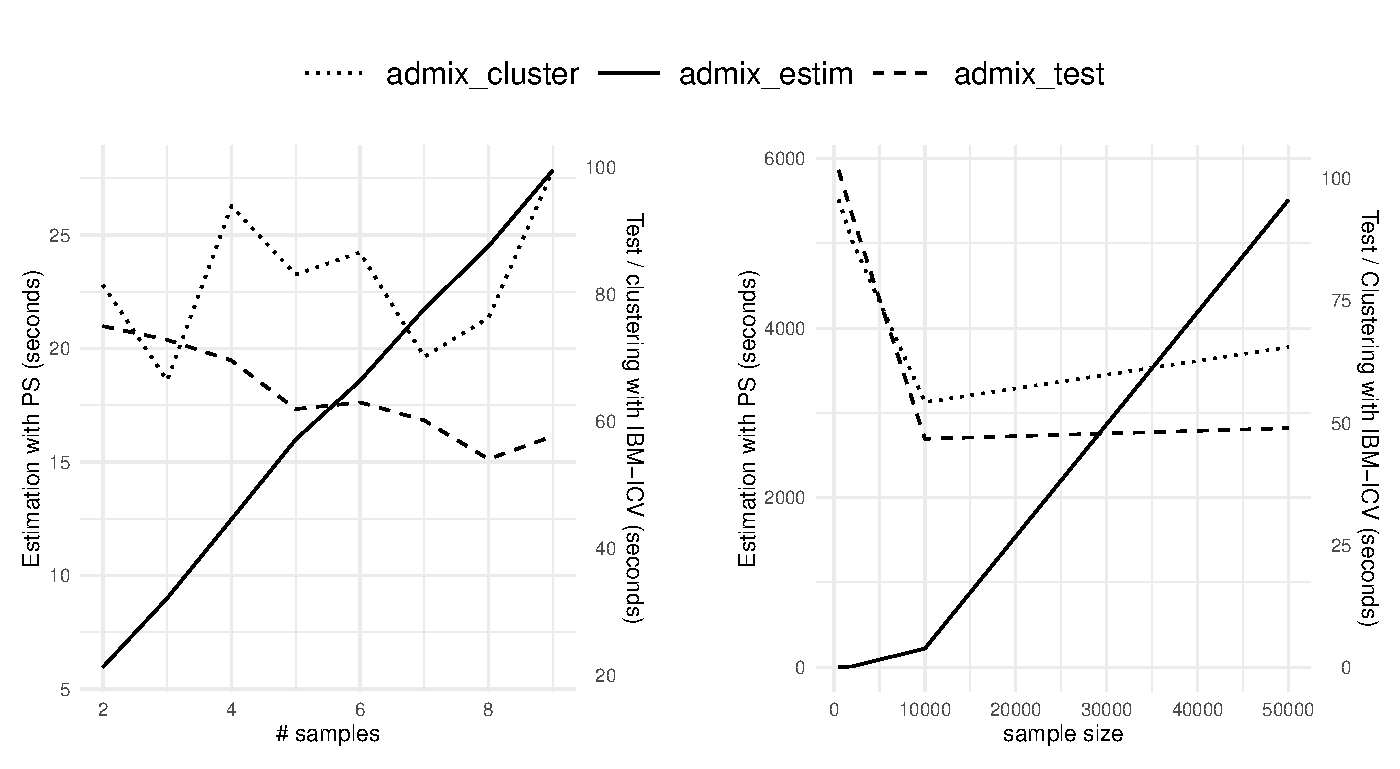
\includegraphics[width=0.9\linewidth,height=0.3\textheight]{compCost} 

}

\caption{Computation time of the three main functions with respect to the number of samples under study (left panel, $n=2000$ fixed) and the sample size (right panel, $K=3$ fixed).}\label{fig:computationCost-latex}
\end{figure}

\section{Practical use of the package}\label{sec:practicalUse}

To make the functionalities of the package as clear as possible, this section has been divided into subsections according to the number of samples the user has to deal with, \emph{i.e.} 1, 2 or \(K\), with \(K > 2\).
We also detail which are the available options depending on the symmetry assumption made (or not) about the unknown component density.

\subsection{The 1-sample case: estimation and test}\label{sec:1sample}

The parameters involved in our simulations for the 1-sample case are stored in Table \ref{tab:admix-simu1-latex}. Values to be estimated are the proportions in the third column, as well as unknown distributions in the fifth one.

\begin{table}[!h]
\centering
\caption{\label{tab:admix-simu1-latex}Simulation parameters in the 1-sample case, with Gaussian-Exponential mixtures.}
\centering
\resizebox{\ifdim\width>\linewidth\linewidth\else\width\fi}{!}{
\fontsize{9}{11}\selectfont
\begin{tabular}[t]{cccccc}
\toprule
 & $n_i$ & $p_i$ & $G_i$ & $F_i$ & Support\\
\midrule
sim1 & 700 & 0.44 & $\mathcal{N}(0,1)$ & $\mathcal{N}(-2,1)$ & $\mathbb{R}$\\
sim2 & 1000 & 0.23 & $\mathcal{E}(3)$ & $\mathcal{E}(1/3)$ & $\mathbb{R}^+$\\
\bottomrule
\end{tabular}}
\end{table}

They refer to two different cases: either the unknown component density is symmetric (\texttt{sim1}) or not (\texttt{sim2}). We also make the support of the distributions change, to show that available methods enable one to deal with such contexts. More precisely, we consider supports on \(\mathbb{R}\) and \(\mathbb{R}^+\).

\subsubsection{Estimation of the mixture proportion assuming a symmetric unknown density}\label{estimation-of-the-mixture-proportion-assuming-a-symmetric-unknown-density}

In the one-sample case and assuming a symmetric unknown density, both \emph{BVdk} and \emph{PS} estimators can be used. In terms of implementation, the user has to set the argument \texttt{est\_method} to the value ``BVdk'' or ``PS'' in \texttt{admix\_estim()}, which calls the appropriate subroutine. If ``BVdk'' is chosen (which is the case below), the function returns the two estimated Euclidean unknown parameters, \emph{i.e.} the estimated unknown weight as well as the estimated unknown location parameter.

For illustration purposes and thanks to the method \texttt{twoComp\_mixt()}, we first simulate a two-component Gaussian mixture where the known component distribution \(G\) in model \eqref{eq:model} is a standard Gaussian distribution, see Table \ref{tab:admix-simu1-latex}. The created object contains the simulated mixture data, as well as the information regarding the generating model. This can be useful when defining the admixture model under consideration in such a simulation framework, through the \texttt{admix\_model()} method.

\begin{verbatim}
# Simulate data: 'f' represents the unknown distribution, and 'g' the known one.
list.comp <- list(f = "norm", g = "norm")
list.param <- list(f = list("mean"=-2, "sd"=1), g = list("mean"=0, "sd"=1))
set.seed(1)
mix1 <- twoComp_mixt(n = 700, weight = 0.44, comp.dist = list(list.comp$f, list.comp$g),
                     comp.param = list(list.param$f, list.param$g))
print(mix1)
\end{verbatim}

\begin{verbatim}
#> 
#> Call:twoComp_mixt(n = 700, weight = 0.44, comp.dist = list(list.comp$f, 
#>     list.comp$g), comp.param = list(list.param$f, list.param$g))
#> 
#> Number of observations: 700 
#> 
#> Simulated data (first 5 obs.): 
#>  1.473881 0.6772685 -1.620037 -2.192798 1.577892
#> Simulated observations coming from the 1st component (first 5 obs.): 
#>  -1.620037 -2.192798 -1.403766 -3.173577 -2.155643
#> Simulated observations coming from the 2nd component (first 5 obs.): 
#>  1.473881 0.6772685 1.577892 -0.1952588 -2.592328
\end{verbatim}

\begin{verbatim}
# Get simulated data, define the admixture model (only 1 known component in real-life)
sim1 <- get_mixture_data(mix1)
admixMod1 <- admix_model(knownComp_dist = "norm",
                         knownComp_param = list("mean" = 0, "sd" = 1))
# Performs estimation with Bordes and Vandekerkhove estimator:
est <- admix_estim(samples = list(sim1), admixMod = list(admixMod1),
                   est_method = 'BVdk', compute_var = TRUE)
print(est)
\end{verbatim}

\begin{verbatim}
#> 
#> Call:
#> admix_estim(samples = list(sim1), admixMod = list(admixMod1), 
#>     est_method = "BVdk", compute_var = TRUE)
#> 
#> Method: BVdk  -  Number of samples: 1 
#> 
#>  sample size mix_weight location var_mix_weight var_location
#>    sim1  700      0.431    -2.10        0.00128      0.01302
\end{verbatim}

The obtained estimates are close to the true values, see Table \ref{tab:admix-simu1-latex}. Moreover, one also gets the information about the variance of the estimators in that estimation approach.

\subsubsection{Estimation of the mixture proportion without the symmetric constraint}\label{estimation-of-the-mixture-proportion-without-the-symmetric-constraint}

In this framework, the only available estimator is the \emph{PS} estimator. The estimation of the unknown proportion is performed using \texttt{admix\_estim()}, setting \texttt{est\_method\ =\ "PS"}. To go further into the analysis, one can use specific arguments in place of the \texttt{...} argument, which are available by typing \texttt{?estim\_PS}. Notably, parameters related to the cross-validation procedure (supposed to make the estimation more robust) can be specified. We now consider the second dataset \texttt{sim2} in Table \ref{tab:admix-simu1-latex}.

\begin{verbatim}
list.comp <- list(f = "exp", g = "exp")
list.param <- list(f = list("rate" = 1/3), g = list("rate" = 3))
mix2 <- twoComp_mixt(n = 1000, weight = 0.23, comp.dist = list(list.comp$f, list.comp$g),
                     comp.param = list(list.param$f, list.param$g))
sim2 <- get_mixture_data(mix2)
admixMod2 <- admix_model(knownComp_dist = mix2$comp.dist[[2]],
                         knownComp_param = mix2$comp.param[[2]])
admix_estim(samples = list(sim2), admixMod = list(admixMod2), est_method = 'PS')
\end{verbatim}

\begin{verbatim}
#> 
#> Call:
#> admix_estim(samples = list(sim2), admixMod = list(admixMod2), 
#>     est_method = "PS")
#> 
#> Method: PS  -  Number of samples: 1 
#> 
#>  sample size mix_weight
#>    sim2 1000      0.208
\end{verbatim}

Again, the mixing weight has been correctly estimated. Note that the asymptotic variance of the estimator is explicitly known with the \emph{BVdk} estimator, which is not the case here.

\subsubsection{Estimation of the decontaminated density}\label{estimation-of-the-decontaminated-density}

Once the estimations of the mixing weight are performed, it is then possible to estimate the decontaminated density as detailed in Section \ref{sec:decontamine}. To illustrate this, we focus on the first admixture model considered in Table \ref{tab:admix-simu1-latex}, with dataset \texttt{sim1}. The following code enables one to get the decontaminated density of the unknown component in admixture \texttt{sim1}, and visualize it in Figure \ref{fig:oneSampleDecontaminDensity}.

\begin{verbatim}
est_weight <- get_mixing_weights(est)
# Build the object related to the decontaminated density:
dec.f <- decontaminated_density(sample1 = sim1, estim.p = est_weight,
                                admixMod = admixMod1)
par(mar = c(3,3,0.5,1.5), cex = 0.7)
plot(x = dec.f, xlim = c(-5,1), ylim = c(0,0.45), main = "")
lines(x = seq(from = -5, to = 1, by = 0.01),
      y = dnorm(seq(from=-5, to=1, by=0.01), mean=-2, sd=1), lty=2)
\end{verbatim}

\begin{figure}

{\centering 
\includegraphics[width=0.35\linewidth,height=0.18\textheight]{milhaud-pommeret-salhi-vandekerkhove_files/figure-latex/oneSampleDecontaminDensity-1} 

}

\caption{Theoretical gaussian density $\mathcal{N}(-2,1)$ (dashed) and decontaminated density (plain).}\label{fig:oneSampleDecontaminDensity}
\end{figure}

As expected, the decontaminated density looks like a standardized Gaussian centered at -2.

\subsubsection{Statistical test}\label{statistical-test}

In the 1-sample case, the implemented test is a \emph{gaussianity test}, called by \texttt{admix\_test()} setting argument \texttt{test\_method} to ``poly''. In addition to the classical inputs of \texttt{admix\_test()}, the user can specify through argument \texttt{...} other additional arguments of the unexported subroutine \texttt{gaussianity\_test()} (see \texttt{?gaussianity\_test}). These arguments are connected to the underlying theory, namely the order to which the expansion of the density is performed and the penalization exponent which appears in the penalization rule (see the parameter \(\lambda\) in Section \ref{sec:testingMeth}). It is thus possible and recommended to play with these arguments, whose default values have been fixed in order to give satisfactory results in most of the situations (without any prior knowledge about the result of the test, the penalty exponent is set to 0.25).

\begin{verbatim}
admix_test(samples = list(sim1), admixMod = list(admixMod1),
           test_method = 'poly', conf_level = 0.95)
\end{verbatim}

\begin{verbatim}
#> 
#>  Gaussianity test for the unknown component distribution
#> 
#> data:  samples[[1]]
#> T = 0.10176, expansion order S = 1, p-value = 0.7497
#> alternative hypothesis: Unknown component of the contamination 
#>                        model is not normally distributed
#> sample estimates:
#>     Weight   Location   Variance 
#>  0.4934484 -1.9588427  1.3772585
\end{verbatim}

Here, the results show that the null hypothesis cannot be rejected, with a p-value about 0.75. This is the expected output since the data \texttt{sim1} were generated according to a two-component Gaussian mixture, see Table \ref{tab:admix-simu1-latex}.

\subsection{The 2-sample case: estimation and test}\label{the-2-sample-case-estimation-and-test}

In contrast with the 1-sample case, the 2-sample setting gives the opportunity to use the \emph{IBM} approach, whether for estimation or testing purposes. Table \ref{tab:admix-simu2-latex} stores the simulation parameters used in the framework of continuous random variables, with symmetric unknown component densities or not. Examples with discrete random variables, only available through the \emph{IBM} approach, are provided further in the current section.

\begin{table}[!h]
\centering
\caption{\label{tab:admix-simu2-latex}Parameters in the two-sample case (K=2), with Gaussian and Exponential distributions.}
\centering
\resizebox{\ifdim\width>\linewidth\linewidth\else\width\fi}{!}{
\fontsize{9}{11}\selectfont
\begin{tabular}[t]{cccccc}
\toprule
 & $n_i$ & $p_i$ & $G_i$ & $F_i$ & Support\\
\midrule
sim3 & 1300 & 0.75 & $\mathcal{E}(1/2)$ & $\mathcal{N}(-3,1)$ & $\mathbb{R}$\\
sim4 & 1500 & 0.47 & $\mathcal{E}(1/4)$ & $\mathcal{N}(-2.2,1)$ & $\mathbb{R}$\\
\midrule
sim5 & 1850 & 0.31 & $\mathcal{N}(-3,1)$ & $\mathcal{E}(1)$ & $\mathbb{R}$\\
sim6 & 2350 & 0.15 & $\mathcal{N}(5,1)$ & $\mathcal{E}(1)$ & $\mathbb{R}$\\
\bottomrule
\end{tabular}}
\end{table}

\subsubsection{Estimation of the mixture proportion assuming a symmetric unknown density}\label{estimation-of-the-mixture-proportion-assuming-a-symmetric-unknown-density-1}

Assuming a symmetric density for the unknown component in the two-sample case does not change anything from Section \ref{sec:1sample}, except that one duplicates the estimation technique over each observed sample and gets the list of estimated unknown parameters. Following this principle, the implementation is very simple in that the new sample is added into the list of samples through the first argument of the function, when everything else remains identical.
We start by simulating the first two models in Table \ref{tab:admix-simu2-latex}, leading to samples \texttt{sim3} and \texttt{sim4}:

\begin{verbatim}
list.comp <- list(f3 = "norm", g3 = "exp", f4 = "norm", g4 = "exp")
list.param <- list(f3 = list("mean"=-3, "sd"=1), g3 = list("rate"=1/2),
                   f4 = list("mean"=-2.2, "sd"=1), g4 = list("rate"=1/4))
mix3 <- twoComp_mixt(n = 1300, weight = 0.75, comp.dist = list(list.comp$f3, list.comp$g3),
                     comp.param = list(list.param$f3, list.param$g3))
mix4 <- twoComp_mixt(n = 1500, weight = 0.47, comp.dist = list(list.comp$f4, list.comp$g4),
                     comp.param = list(list.param$f4, list.param$g4))
sim3 <- get_mixture_data(mix3) ; sim4 <- get_mixture_data(mix4)
admixMod3 <- admix_model(knownComp_dist = mix3$comp.dist[[2]],
                         knownComp_param = mix3$comp.param[[2]])
admixMod4 <- admix_model(knownComp_dist = mix4$comp.dist[[2]],
                         knownComp_param = mix4$comp.param[[2]])
admix_estim(samples = list(sim3, sim4), admixMod = list(admixMod3, admixMod4),
            est_method = 'BVdk', compute_var = FALSE)
\end{verbatim}

\begin{verbatim}
#> 
#> Call:
#> admix_estim(samples = list(sim3, sim4), admixMod = list(admixMod3, 
#>     admixMod4), est_method = "BVdk", compute_var = FALSE)
#> 
#> Method: BVdk  -  Number of samples: 2 
#> 
#>  sample size mix_weight location
#>    sim3 1300      0.737    -2.97
#>    sim4 1500      0.487    -2.13
\end{verbatim}

We can see that the estimators are quite close to the true unknown values (see Table \ref{tab:admix-simu2-latex}), respectively \((p_3, \mu_3) = (0.75, -3)\) and \((p_4, \mu_4) = (0.47, -2.2)\).

\subsubsection{Estimation of the mixture proportion without the symmetric constraint}\label{estimation-of-the-mixture-proportion-without-the-symmetric-constraint-1}

Here, there are two possibilities: either duplicate the procedure described in Section \ref{sec:1sample} using the \emph{PS} estimator, or consider the \emph{IBM} approach. In the first case, simply add the new sample to the list of existing samples where unknown proportions have to be estimated. We now work with samples \texttt{sim5} and \texttt{sim6} in Table \ref{tab:admix-simu2-latex}:

\begin{verbatim}
list.comp <- list(f5 = "exp", g5 = "norm", f6 = "exp", g6 = "norm")
list.param <- list(f5 = list("rate"=1), g5 = list("mean"=-3, "sd"=1),
                   f6 = list("rate"=1), g6 = list("mean"=5, "sd"=1))
mix5 <- twoComp_mixt(n = 1850, weight = 0.31, comp.dist = list(list.comp$f5, list.comp$g5),
                     comp.param = list(list.param$f5, list.param$g5))
mix6 <- twoComp_mixt(n = 2350, weight = 0.15, comp.dist = list(list.comp$f6, list.comp$g6),
                     comp.param = list(list.param$f6, list.param$g6))
sim5 <- get_mixture_data(mix5) ; sim6 <- get_mixture_data(mix6)
admixMod5 <- admix_model(knownComp_dist = mix5$comp.dist[[2]],
                         knownComp_param = mix5$comp.param[[2]])
admixMod6 <- admix_model(knownComp_dist = mix6$comp.dist[[2]],
                         knownComp_param = mix6$comp.param[[2]])
admix_estim(samples = list(sim5,sim6), admixMod = list(admixMod5,admixMod6),
            est_method = 'PS', method = "fixed")
\end{verbatim}

\begin{verbatim}
#> 
#> Call:
#> admix_estim(samples = list(sim5, sim6), admixMod = list(admixMod5, 
#>     admixMod6), est_method = "PS", method = "fixed")
#> 
#> Method: PS  -  Number of samples: 2 
#> 
#>  sample size mix_weight
#>    sim5 1850      0.315
#>    sim6 2350      0.147
\end{verbatim}

Once again, the parameters are consistently estimated (0.315 versus 0.31, and 0.147 versus 0.15).

The alternative, which consists in using the \emph{IBM} estimator, gives consistent results if the unknown components of the two admixture models have the same distribution (and provided that the two known components have different distributions). If the two known components are identical, the estimated ratio of weights is consistent towards the actual ratio of weights (instead of the weights themselves), see the Supplementary Material in \citet{Milhaud+Pommeret+Salhi+Vandekerkhove:2023}. Given our parameters for simulating \texttt{sim5} and \texttt{sim6}, we have two different known components and two similar unknown components, which should thus lead to consistent estimators. \emph{However, the user must keep in mind that obtained estimators using IBM are most of the time inconsistent, since there is no reason for the two unknown components to share the same distribution}. To perform the estimation, simply call \texttt{admix\_estim()} with argument \texttt{est\_method} set to ``IBM'', which calls in practice the unexported subroutine \texttt{estim\_IBM()} that estimates the unknown proportions of the contaminating components.

\begin{verbatim}
est <- admix_estim(samples = list(sim5, sim6), admixMod = list(admixMod5, admixMod6),
                   est_method = 'IBM', compute_var = TRUE)
print(est)
\end{verbatim}

\begin{verbatim}
#> 
#> Call:
#> admix_estim(samples = list(sim5, sim6), admixMod = list(admixMod5, 
#>     admixMod6), est_method = "IBM", compute_var = TRUE)
#> 
#> Method: IBM  -  Pairwise estimation
#> 
#>          pair size_1st size_2nd mix_weight_1st var_1st mix_weight_2nd var_2nd
#>  sim5 vs sim6     1850     2350          0.318 0.00014          0.149   7e-05
\end{verbatim}

We can check whether using this estimator in the general case leads to unreliable estimates, due to different unknown component distributions:

\begin{verbatim}
admix_estim(samples = list(sim3,sim4), admixMod = list(admixMod3,admixMod4),
            est_method = 'IBM', compute_var = FALSE)
\end{verbatim}

\begin{verbatim}
#> 
#> Call:
#> admix_estim(samples = list(sim3, sim4), admixMod = list(admixMod3, 
#>     admixMod4), est_method = "IBM", compute_var = FALSE)
#> 
#> Method: IBM  -  Pairwise estimation
#> 
#>          pair size_1st size_2nd mix_weight_1st var_1st mix_weight_2nd var_2nd
#>  sim3 vs sim4     1300     1500          1.356      NA          0.720      NA
\end{verbatim}

Here, the estimated weight of the unknown component distribution in the first sample is unrealistic, making it clear that the estimate is unreliable. On the other hand, it is possible to observe a realistic weight estimate while in this configuration. The user should therefore \emph{never} choose the \emph{IBM} estimation method without performing the test for equality of unknown component distributions before. In full generality, it is safer to use the \emph{PS} estimator for robust estimation purposes.

\subsubsection{Estimate the decontaminated densities}\label{estimate-the-decontaminated-densities}

In the two-sample case, both decontaminated densities can be plotted on the same graph, which is useful to get a visual comparison. To this aim, it is recommended to use the \texttt{plot()} method designed for objects of class \texttt{decontaminated\_density}. In Figure \ref{fig:2sampleDecontaminDensit}, we compare the decontaminated densities obtained from admixture models \texttt{sim5} and \texttt{sim6}.

\begin{figure}

{\centering 
\includegraphics[width=0.7\linewidth,height=0.2\textheight]{milhaud-pommeret-salhi-vandekerkhove_files/figure-latex/2sampleDecontaminDensit-1} 

}

\caption{Decontaminated densities and cdfs obtained from samples sim5 (plain) and sim6 (dashed).}\label{fig:2sampleDecontaminDensit}
\end{figure}

Clearly, these decontaminated densities look similar (which is expected as they are both exponentially distributed with mean 1, see Table \ref{tab:admix-simu2-latex}). The black curve is based on more observations associated with the unknown component (\(0.31*1850\)), leading to a more accurate estimate. Due to the inversion formula \eqref{eq:decontaminatedCDF}, the imperfect estimated proportion and the negative mean of the Gaussian known component, the support of the estimated decontaminated density function is on the real line. The bumps appearing on the red curve may come from the inversion formula applied to some kernel density estimator of the observations that can sometimes enhance some peaks depending on the bandwidth choice. To balance this feeling we also provide on the right side of Figure \ref{fig:2sampleDecontaminDensit} the decontaminated cdf which sticks overall pretty well to the true unknown cdf. We now show how to formally test their equality.

\subsubsection{Statistical test}\label{statistical-test-1}

Testing for equality between the two unknown component distributions can be made through two approaches: comparison of expansion coefficients of the corresponding densities in some orthonormal basis, or using the inner convergence property (see Section \ref{sec:testingMeth}). The function dedicated to performing this statistical test is \texttt{admix\_test()}. Depending on the specification of its arguments, either the unexported subroutines \texttt{orthobasis\_test()} or \texttt{IBM\_k\_samples\_test()} is called.
We first show how to perform the test based on polynomial expansions of the densities, setting argument \texttt{test\_method} to the value ``poly'' and testing the equality of unknown components in \texttt{sim3} and \texttt{sim4} models (see Table \ref{tab:admix-simu2-latex}).

\begin{verbatim}
admix_test(samples = list(sim3,sim4), admixMod = list(admixMod3,admixMod4),
           test_method = "poly", conf_level = 0.95, support = "Real")
\end{verbatim}

\begin{verbatim}
#> 
#>  Equality test of unknown distributions with polynomial expansions of
#>  pdfs
#> 
#> data:  samples
#> T = 5.1288, expansion order S = 1, p-value = 0.02353
#> alternative hypothesis: Distributions of unknown components involved 
#>                         in the contamination models are different
\end{verbatim}

The tests provide consistent results, in that \texttt{sim3} and \texttt{sim4} were admixture models with close (but different) unknown component distributions. The test is performed with default values for all arguments, including hidden arguments of the internal subroutine \texttt{orthobasis\_test()} which is called. In practice, we advise using this test only if the initial sample sizes are large enough. Indeed, the procedure splits the initial samples into subsamples to decorrelate the various estimators involved in the test strategy, which leads to lowering the size of the data considered for each estimator plugged into the test statistic.
In addition, we recommend avoiding using this testing strategy in the general case, since conditions that guarantee the asymptotic properties of this test are usually not met. Indeed, on the one hand the symmetry of the unknown component density is sometimes hard to figure out, which should prevent using the \emph{BVdk} estimator (through argument \texttt{est\_method}). On the other hand, using the \emph{PS} estimator plugged into the test statistic is in theory not allowed, since the latter estimator is not square-root \(\sqrt{n}\)-consistent (see Section \ref{sec:testingMeth}).

An alternative to test the equality of the two unknown components is therefore to use the \emph{i}nner \emph{c}on\emph{v}ergence property (\emph{icv}), which remains valid whatever the context. In this case, computations can be accelerated thanks to the package \pkg{parallel} that allows for parallel computing. One of the most important arguments for the reliability of the test is \texttt{n\_sim\_tab} (with default value set to 100), which controls the number of simulated realizations of the stochastic integral involved in the tabulation of the quantile to be tested against (see Section \ref{sec:testingMeth}). The higher this argument is, the more reliable the test should be. Not surprisingly, increasing \texttt{n\_sim\_tab} causes a much longer computation time. In terms of implementation, setting the argument \texttt{test\_method} to ``icv'' in the generic function \texttt{admix\_test()} calls the unexported subroutine \texttt{IBM\_k\_samples\_test()} (see \texttt{?IBM\_k\_samples\_test} for the list of potential specific arguments in place of \texttt{...} in \texttt{admix\_test()}). We first test the equality of unknown component distributions between \texttt{sim3} and \texttt{sim4}, and then between \texttt{sim5} and \texttt{sim6}.

\begin{verbatim}
admix_test(samples = list(sim3,sim4), admixMod = list(admixMod3,admixMod4),
           test_method = "icv", conf_level = 0.95, n_sim_tab = 50,
           parallel = TRUE, n_cpu = 8)
\end{verbatim}

\begin{verbatim}
#> 
#>  Equality test of unknown distributions using Inner ConVergence regime
#> 
#> data:  samples
#> T = 2.2896, p-value = 1e-12
#> alternative hypothesis: Distributions of unknown components involved 
#>                         in the contamination models are different
\end{verbatim}

\begin{verbatim}
admix_test(samples = list(sim5,sim6), admixMod = list(admixMod5,admixMod6),
           test_method = "icv", conf_level = 0.95, n_sim_tab = 50,
           parallel = TRUE, n_cpu = 8)
\end{verbatim}

\begin{verbatim}
#> 
#>  Equality test of unknown distributions using Inner ConVergence regime
#> 
#> data:  samples
#> T = 1.0315, p-value = 0.9773
#> alternative hypothesis: Distributions of unknown components involved 
#>                         in the contamination models are different
\end{verbatim}

Again, the results of the tests are consistent with the nature of the samples (see Table \ref{tab:admix-simu2-latex}). In particular, the first equality test between \texttt{sim3} and \texttt{sim4} leads to unreliable estimates of the weights, causing the automatic rejection of the null hypothesis. Now, one can introduce some examples based on other types of support, since the \emph{IBM} approach as well as the \emph{ICV} property are suitable for every kind of observation. More precisely, the next section considers either continuous or discrete distributions.

\subsubsection{Estimations and tests on other supports with IBM}\label{estimations-and-tests-on-other-supports-with-ibm}

In Table \ref{tab:simParam2-discrete-latex}, we store the information about simulation parameters for distributions supported on discrete or bounded supports. This way, we show that the package covers a large panel of potential applications. For conciseness, we do not explore here a wide range of situations, but the user is encouraged to play with different distributions and settings (equality or not of the unknown component distributions).

\begin{table}[!h]
\centering
\caption{\label{tab:simParam2-discrete-latex}Parameters in the 2-sample case, with other support types (involving Binomial, Poisson, Negative Binomial, Uniform and Beta distributions).}
\centering
\resizebox{\ifdim\width>\linewidth\linewidth\else\width\fi}{!}{
\fontsize{9}{11}\selectfont
\begin{tabular}[t]{cccccc}
\toprule
 & $n_i$ & $p_i$ & $G_i$ & $F_i$ & Support\\
\midrule
sim7 & 550 & 0.40 & $\mathcal{B}(10,0.4)$ & $\mathcal{P}(2)$ & $\mathbb{N}$\\
sim8 & 900 & 0.25 & $\mathcal{NB}(10,0.9)$ & $\mathcal{P}(2)$ & $\mathbb{N}$\\
\midrule
sim9 & 600 & 0.33 & $\mathcal{U}([0,1])$ & $\mathcal{B}eta(1.2,5)$ & $[0,1]$\\
sim10 & 900 & 0.18 & $\mathcal{U}([0,2])$ & $\mathcal{B}eta(1.2,5)$ & $[0,2]$\\
\bottomrule
\end{tabular}}
\end{table}

Firstly, let us perform some estimations and tests on \(\mathbb{N}\)-discrete support, considering the first two models in Table \ref{tab:simParam2-discrete-latex} leading to samples \texttt{sim7} and \texttt{sim8}.

\begin{verbatim}
list.comp <- list(f7 = "pois", g7 = "binom", f8 = "pois", g8 = "nbinom")
list.param <- list(f7 = list("lambda"=2), g7 = list("size"=10, "prob"=0.4),
                   f8 = list("lambda"=2), g8 = list("size"=10, "prob"=0.9))
mix7 <- twoComp_mixt(n = 550, weight = 0.4, comp.dist = list(list.comp$f7, list.comp$g7),
                     comp.param = list(list.param$f7, list.param$g7))
mix8 <- twoComp_mixt(n = 900, weight = 0.25, comp.dist = list(list.comp$f8, list.comp$g8),
                     comp.param = list(list.param$f8, list.param$g8))
sim7 <- get_mixture_data(mix7) ; sim8 <- get_mixture_data(mix8)
admixMod7 <- admix_model(knownComp_dist = mix7$comp.dist[[2]],
                         knownComp_param = mix7$comp.param[[2]])
admixMod8 <- admix_model(knownComp_dist = mix8$comp.dist[[2]],
                         knownComp_param = mix8$comp.param[[2]])
admix_test(samples = list(sim7,sim8), admixMod = list(admixMod7,admixMod8),
           test_method = 'icv', n_sim_tab = 50, parallel = T, n_cpu = 8)
\end{verbatim}

\begin{verbatim}
#> 
#>  Equality test of unknown distributions using Inner ConVergence regime
#> 
#> data:  samples
#> T = 0.29595, p-value = 0.96
#> alternative hypothesis: Distributions of unknown components involved 
#>                         in the contamination models are different
\end{verbatim}

The test did not reject the equality between \texttt{sim7} and \texttt{sim8}, which is in line with reality. Knowing that the null hypothesis has not been rejected, we now estimate the proportions with the \emph{IBM} method:

\begin{verbatim}
admix_estim(samples = list(sim7,sim8), admixMod = list(admixMod7,admixMod8), 
            est_method = "IBM")
\end{verbatim}

\begin{verbatim}
#> 
#> Call:
#> admix_estim(samples = list(sim7, sim8), admixMod = list(admixMod7, 
#>     admixMod8), est_method = "IBM")
#> 
#> Method: IBM  -  Pairwise estimation
#> 
#>          pair size_1st size_2nd mix_weight_1st var_1st mix_weight_2nd var_2nd
#>  sim7 vs sim8      550      900          0.419      NA          0.270      NA
\end{verbatim}

Secondly we are interested in finite bounded support, see the third and fourth models (\texttt{sim9} and \texttt{sim10}) in Table \ref{tab:simParam2-discrete-latex}:

\begin{verbatim}
list.comp <- list(f9 = "beta", g9 = "unif", f10 = "beta", g10 = "unif")
list.param <- list(f9= list("shape1"=1.2, "shape2"=5, "ncp"=0), g9= list("min"=0, "max"=1),
                   f10= list("shape1"=1.2, "shape2"=5, "ncp"=0), g10= list("min"=0, "max"=2))
mix9 <- twoComp_mixt(n = 600, weight = 0.33, comp.dist = list(list.comp$f9, list.comp$g9),
                     comp.param = list(list.param$f9, list.param$g9))
mix10 <- twoComp_mixt(n = 900, weight = 0.18, comp.dist = list(list.comp$f10, list.comp$g10),
                      comp.param = list(list.param$f10, list.param$g10))
sim9 <- get_mixture_data(mix9) ; sim10 <- get_mixture_data(mix10)
admixMod9 <- admix_model(knownComp_dist = mix9$comp.dist[[2]],
                         knownComp_param = mix9$comp.param[[2]])
admixMod10 <- admix_model(knownComp_dist = mix10$comp.dist[[2]],
                          knownComp_param = mix10$comp.param[[2]])
admix_test(samples=list(sim9,sim10), admixMod=list(admixMod9,admixMod10),
           test_method = 'icv', n_sim_tab = 50, parallel = TRUE, n_cpu = 8)
\end{verbatim}

\begin{verbatim}
#> 
#>  Equality test of unknown distributions using Inner ConVergence regime
#> 
#> data:  samples
#> T = 1.186, p-value = 1
#> alternative hypothesis: Distributions of unknown components involved 
#>                         in the contamination models are different
\end{verbatim}

Once again, the results are consistent in that the equality of unknown components is not rejected. We can conclude that whatever the support considered in our examples, the results meet our performance expectations.

\subsection{The K-sample case: estimation, test and clustering}\label{the-k-sample-case-estimation-test-and-clustering}

In the \(K\)-sample framework, another question arises: do some of the \(K\) samples share the same unknown component distribution, creating possible clusters? To proceed to such experiments, Table \ref{tab:simParamK-latex} introduces the simulation parameters in the 3-sample case. Estimations, tests and clustering are performed on either continuous or discrete supports.

\begin{table}[!h]
\centering
\caption{\label{tab:simParamK-latex}Simulation parameters for estimations and tests in the $K$-sample case.}
\centering
\fontsize{9}{11}\selectfont
\begin{tabular}[t]{lllllll}
\toprule
 & $K$ & $n_i$ & $p_i$ & $G_i$ & $F_i$ & Support\\
\midrule
sim1 &  & 3500 & 0.70 & $\mathcal{E}(1/4)$ & $\mathcal{N}(1,1)$ & $\mathbb{R}$\\
sim2 & 3 & 5000 & 0.40 & $\mathcal{E}(1/3)$ & $\mathcal{N}(1,1.3)$ & $\mathbb{R}$\\
sim3 &  & 3000 & 0.55 & $\mathcal{G}(10,1/3)$ & $\mathcal{N}(1,1)$ & $\mathbb{R}$\\
\midrule
sim4 &  & 3000 & 0.70 & $\mathcal{B}(10,0.4)$ & $\mathcal{P}(12)$ & $\mathbb{N}$\\
sim5 & 3 & 3500 & 0.50 & $\mathcal{NB}(10,0.9)$ & $\mathcal{P}(12)$ & $\mathbb{N}$\\
sim6 &  & 4000 & 0.30 & $\mathcal{P}(1)$ & $\mathcal{P}(12)$ & $\mathbb{N}$\\
\bottomrule
\end{tabular}
\end{table}

\subsubsection{Estimation of the unknown quantities}\label{estimation-of-the-unknown-quantities}

Given that the \emph{IBM} procedure provides accurate estimates of the unknown weights only when the unknown components of the admixture models are tested to be equal, and that the \emph{BVdk} estimator requires shape constraints about the unknown component densities (symmetry), the privileged procedure is the \emph{PS} estimator in full generality. It is thus deployed in each sample, and we now give an example based on three samples (\(K=3\)) with simulation parameters stored in Table \ref{tab:simParamK-latex}.

\begin{verbatim}
# Simulation of data (3 samples) with continuous random variables:
comp_c <- list(f1 = "norm", g1 = "exp", f2 = "norm", g2 = "exp",
               f3 = "norm", g3 = "gamma")
param_c <- list(f1 = list("mean"=1,"sd"=1), g1 = list("rate"=1/4),
                f2 = list("mean"=1,"sd"=1.3), g2 = list("rate"=1/3),
                f3 = list("mean"=1,"sd"=1), g3 = list("shape"=10,"scale"=1/3))
mix1 <- twoComp_mixt(n = 3500, weight = 0.7, comp.dist = list(comp_c$f1, comp_c$g1),
                     comp.param = list(param_c$f1, param_c$g1))
mix2 <- twoComp_mixt(n = 5000, weight = 0.4, comp.dist = list(comp_c$f2, comp_c$g2),
                     comp.param = list(param_c$f2, param_c$g2))
mix3 <- twoComp_mixt(n = 3000, weight = 0.55, comp.dist = list(comp_c$f3, comp_c$g3),
                     comp.param = list(param_c$f3, param_c$g3))
sim1 <- get_mixture_data(mix1) ; sim2 <- get_mixture_data(mix2)
sim3 <- get_mixture_data(mix3)
admixMod1 <- admix_model(knownComp_dist = mix1$comp.dist[[2]],
                         knownComp_param = mix1$comp.param[[2]])
admixMod2 <- admix_model(knownComp_dist = mix2$comp.dist[[2]],
                         knownComp_param = mix2$comp.param[[2]])
admixMod3 <- admix_model(knownComp_dist = mix3$comp.dist[[2]],
                         knownComp_param = mix3$comp.param[[2]])
# Estimation of unknown mixing weights (Patra and Sen estimator):
admix_estim(samples = list(sim1, sim2, sim3), 
            admixMod = list(admixMod1, admixMod2, admixMod3), est_method = 'PS')
\end{verbatim}

\begin{verbatim}
#> 
#> Call:
#> admix_estim(samples = list(sim1, sim2, sim3), admixMod = list(admixMod1, 
#>     admixMod2, admixMod3), est_method = "PS")
#> 
#> Method: PS  -  Number of samples: 3 
#> 
#>  sample size mix_weight
#>    sim1 3500      0.673
#>    sim2 5000      0.368
#>    sim3 3000      0.567
\end{verbatim}

\begin{verbatim}
# Simulation of data (3 samples) with discrete random variables:
comp_d <- list(f1 = "pois", g1 = "binom", f2 = "pois", 
               g2 = "nbinom", f3 = "pois", g3 = "pois")
param_d <- list(f1 = list("lambda"=12), g1 = list("size"=10, "prob"=0.4),
                f2 = list("lambda"=12), g2 = list("size"=10, "prob"=0.9),
                f3 = list("lambda" = 12), g3 = list("lambda" = 1))
mix4 <- twoComp_mixt(n = 3000, weight = 0.7, comp.dist = list(comp_d$f1, comp_d$g1),
                     comp.param = list(param_d$f1, param_d$g1))
mix5 <- twoComp_mixt(n = 3500, weight = 0.5, comp.dist = list(comp_d$f2, comp_d$g2),
                     comp.param = list(param_d$f2, param_d$g2))
mix6 <- twoComp_mixt(n = 4000, weight = 0.3, comp.dist = list(comp_d$f3, comp_d$g3),
                     comp.param = list(param_d$f3, param_d$g3))
sim4 <- get_mixture_data(mix4) ; sim5 <- get_mixture_data(mix5)
sim6 <- get_mixture_data(mix6)
admixMod4 <- admix_model(knownComp_dist = mix4$comp.dist[[2]],
                         knownComp_param = mix4$comp.param[[2]])
admixMod5 <- admix_model(knownComp_dist = mix5$comp.dist[[2]],
                         knownComp_param = mix5$comp.param[[2]])
admixMod6 <- admix_model(knownComp_dist = mix6$comp.dist[[2]],
                         knownComp_param = mix6$comp.param[[2]])
# Estimation of unknown mixing weights (Patra and Sen estimator):
admix_estim(samples = list(sim4, sim5, sim6), 
            admixMod = list(admixMod4, admixMod5, admixMod6), est_method = 'PS')
\end{verbatim}

\begin{verbatim}
#> 
#> Call:
#> admix_estim(samples = list(sim4, sim5, sim6), admixMod = list(admixMod4, 
#>     admixMod5, admixMod6), est_method = "PS")
#> 
#> Method: PS  -  Number of samples: 3 
#> 
#>  sample size mix_weight
#>    sim4 3000      0.680
#>    sim5 3500      0.484
#>    sim6 4000      0.323
\end{verbatim}

Both \emph{BVdk} and \emph{PS} should provide consistent estimates for the first three admixtures since we are in the context of symmetric unknown densities; see Table \ref{tab:simParamK-latex}. By contrast, one could not trust the estimates obtained using IBM, since the \(F_i\)'s do not all have the same distribution. In fact, a pairwise IBM estimation based on comparing the first and third samples should lead to consistent estimates since unknown component distributions are identical in these two samples. However, at this stage, we are not supposed to have this information.

\subsubsection{Testing}\label{testing}

In the \(K\)-sample framework, with \(K>2\), the unexported subroutine \texttt{IBM\_k\_samples\_test()} is systematically called by \texttt{admix\_test()} (setting argument \texttt{test\_method} to ``icv''). To increase the reliability of the test, the argument \texttt{n\_sim\_tab} plays a key role: the higher it is, the more reliable the conclusion of the test is. If the user can perform parallel computing with multiple cpus, we recommend setting this argument at least to 100 (default value). Moreover, another argument is important in finite sample applications where the sample sizes are unbalanced (or with very limited size): \texttt{tune\_penalty}. This boolean, set by default to TRUE, allows one to considerably improve the quality of the testing methodology, see \citep{Milhaud+Pommeret+Salhi+Vandekerkhove:2024b}. Here, we test the equality of the three unknown distributions involved in the three models of Table \ref{tab:simParamK-latex}, either with continuous or discrete random variables.

\begin{verbatim}
# Test whether the first three admixtures share the same contaminating phenomenon:
admix_test(samples = list(sim1, sim2, sim3), admixMod = list(admixMod1, admixMod2, admixMod3),
           test_method = "icv", conf_level = 0.95, n_sim_tab = 50, parallel = T, n_cpu = 8)
\end{verbatim}

\begin{verbatim}
#> 
#>  Equality test of unknown distributions using Inner ConVergence regime
#> 
#> data:  samples
#> U = 1.3562, number of terms S = 3, p-value < 2.2e-16
#> alternative hypothesis: Distributions of unknown components involved 
#>                         in the contamination models are different
\end{verbatim}

\begin{verbatim}
# Same task for the last three admixtures:
admix_test(samples = list(sim4, sim5, sim6), admixMod = list(admixMod4, admixMod5, admixMod6),
           test_method = "icv", conf_level = 0.95, n_sim_tab = 50, parallel = T, n_cpu = 8)
\end{verbatim}

\begin{verbatim}
#> 
#>  Equality test of unknown distributions using Inner ConVergence regime
#> 
#> data:  samples
#> U = 0.11758, number of terms S = 1, p-value = 0.96
#> alternative hypothesis: Distributions of unknown components involved 
#>                         in the contamination models are different
\end{verbatim}

The result of these 3-sample tests is in line with what is expected, \emph{i.e.} one rejects the null hypothesis in the continuous case and cannot reject it in the discrete case.
Finally, the natural question is now: how can this \(k\)-sample testing method be used in order to process a model-based clustering of the sample collection?

\subsubsection{Clustering}\label{clustering-1}

The clustering strategy available in the package \CRANpkg{admix} is grounded on the \(k\)-sample testing problem. The generic function of the package dedicated to the clustering of various contaminated samples is the method \texttt{admix\_cluster()}. In this example, we draw four two-component mixture distributions on \(\mathbb{R}^+\) (Exponential-Gamma and Gamma-Gamma distributions), with asymmetric densities. We also draw four two-component multinomial mixtures for the discrete case. The parameters involved in those simulations are available in Table \ref{tab:storyParam-latex}.

\begin{table}[!h]
\centering
\caption{\label{tab:storyParam-latex}Parameters used for simulations (pop1 to pop4 for mixtures of continuous random variables, and pop5 to pop8 in the discrete case), with Gamma, Exponential, and Multinomial distributions.}
\centering
\resizebox{\ifdim\width>\linewidth\linewidth\else\width\fi}{!}{
\begin{tabular}[t]{ccccccccc}
\toprule
 & pop1 & pop2 & pop3 & pop4 & pop5 & pop6 & pop7 & pop8\\
\midrule
$n_i$ & 5600 & 6000 & 4500 & 4000 & 5000 & 3500 & 4000 & 5000\\
$p_i$ & 0.3 & 0.2 & 0.6 & 0.8 & 0.7 & 0.6 & 0.45 & 0.3\\
$F_i$ & $\mathcal{G}(16,4)$ & $\mathcal{G}(14,2)$ & $\mathcal{G}(16,4)$ & $\mathcal{G}(14,2)$ & $\mathcal{M}(0.25,0.5,0.25)$ & $\mathcal{M}(0.25,0.5,0.25)$ & $\mathcal{M}(0.1,0.8,0.1)$ & $\mathcal{M}(0.25,0.5,0.25)$\\
$G_i$ & $\mathcal{E}(1/4)$ & $\mathcal{E}(1/5)$ & $\mathcal{G}(12,0.5)$ & $\mathcal{E}(1/7)$ & $\mathcal{M}(0.8,0.1,0.1)$ & $\mathcal{M}(0.3,0.3,0.4)$ & $\mathcal{M}(0.5,0.3,0.2)$ & $\mathcal{M}(0.1,0.7,0.2)$\\
\bottomrule
\end{tabular}}
\end{table}

First, initialize the parameters and draw simulations of the four finite mixture models:

\begin{verbatim}
# Simulation of Gamma-Exponential / Gamma-Gamma mixtures:
comp <- list(f1 = "gamma", g1 = "exp", f2 = "gamma", g2 = "exp",
             f3 = "gamma", g3 = "gamma", f4 = "gamma", g4 = "exp")
param <- list(f1 = list("shape"=16, "scale"=1/4), g1 = list("rate" = 1/4),
              f2 = list("shape"=14, "scale"=1/2), g2 = list("rate" = 1/5),
              f3=list("shape"=16,"scale"=1/4), g3=list("shape"=12,"scale"=1/2),
              f4 = list("shape"=14, "scale"=1/2), g4 = list("rate" = 1/7))
mix1 <- twoComp_mixt(n = 5600, weight = 0.3, comp.dist = list(comp$f1,comp$g1),
                     comp.param = list(param$f1,param$g1))
mix2 <- twoComp_mixt(n = 6000, weight = 0.2, comp.dist = list(comp$f2,comp$g2),
                     comp.param = list(param$f2,param$g2))
mix3 <- twoComp_mixt(n = 4500, weight = 0.6, comp.dist = list(comp$f3,comp$g3),
                     comp.param = list(param$f3,param$g3))
mix4 <- twoComp_mixt(n = 4000, weight = 0.8, comp.dist = list(comp$f4,comp$g4),
                     comp.param = list(param$f4,param$g4))
# Simulation of samples with mixtures of multinomial random variables:
comp_d <- list(f1 = "multinom", g1 = "multinom", f2 = "multinom", g2 = "multinom", 
               f3 = "multinom", g3 = "multinom", f4 = "multinom", g4 = "multinom")
param_d <- list(f1 = list("size" = 1, "prob" = c(0.25,0.5,0.25)), 
                g1 = list("size" = 1, "prob" = c(0.8,0.1,0.1)),
                f2 = list("size" = 1, "prob" = c(0.25,0.5,0.25)), 
                g2 = list("size" = 1, "prob" = c(0.3,0.3,0.4)),
                f3 = list("size" = 1, "prob" = c(0.7,0.1,0.2)), 
                g3 = list("size" = 1, "prob" = c(0.5,0.3,0.2)),
                f4 = list("size" = 1, "prob" = c(0.25,0.5,0.25)), 
                g4 = list("size" = 1, "prob" = c(0.1,0.7,0.2)))
mix5 <- twoComp_mixt(n = 12200, weight = 0.55, comp.dist = list(comp_d$f1, comp_d$g1),
                     comp.param = list(param_d$f1, param_d$g1))
mix6 <- twoComp_mixt(n = 11300, weight = 0.75, comp.dist = list(comp_d$f2, comp_d$g2),
                     comp.param = list(param_d$f2, param_d$g2))
mix7 <- twoComp_mixt(n = 15000, weight = 0.45, comp.dist = list(comp_d$f3, comp_d$g3),
                     comp.param = list(param_d$f3, param_d$g3))
mix8 <- twoComp_mixt(n = 17000, weight = 0.42, comp.dist = list(comp_d$f4, comp_d$g4),
                     comp.param = list(param_d$f4, param_d$g4))
\end{verbatim}

At this stage, one can observe the distributions displayed in Figure \ref{fig:visualizeToy}.

\begin{figure}

{\centering 
\includegraphics[width=0.99\linewidth,height=0.3\textheight]{milhaud-pommeret-salhi-vandekerkhove_files/figure-latex/visualizeToy-1} 

}

\caption{Distribution of simulated data (left: continuous case - right: discrete case, see Table 9).}\label{fig:visualizeToy}
\end{figure}

Can we cluster some of the unknown random sources \(F_i\)? At first sight and without any other information than the observed distributions and the known \(G_i\)'s, it seems impossible to decide which populations could share the same unknown components. In particular, the third population, showing an unimodal density, seems very different from the others. However, looking at Table \ref{tab:storyParam-latex}, it comes out that the right populations to cluster together (common contamination) are in fact populations 1 and 3, and populations 2 and 4. This shows that it is definitely not trivial to correctly discover the right clusters.
We now look for possible clusters among them. The best in this case is to use as many CPUs as possible to speed up the process, since this step is computationally intensive (it requires performing multiple tests):

\begin{verbatim}
# clustering the continuous contamination models:
admixMod1 <- admix_model(knownComp_dist = mix1$comp.dist[[2]],
                         knownComp_param = mix1$comp.param[[2]])
admixMod2 <- admix_model(knownComp_dist = mix2$comp.dist[[2]],
                         knownComp_param = mix2$comp.param[[2]])
admixMod3 <- admix_model(knownComp_dist = mix3$comp.dist[[2]],
                         knownComp_param = mix3$comp.param[[2]])
admixMod4 <- admix_model(knownComp_dist = mix4$comp.dist[[2]],
                         knownComp_param = mix4$comp.param[[2]])
pop1 <- get_mixture_data(mix1) ; pop2 <- get_mixture_data(mix2)
pop3 <- get_mixture_data(mix3) ; pop4 <- get_mixture_data(mix4)
admix_cluster(samples = list(pop1, pop2, pop3, pop4),
              admixMod = list(admixMod1, admixMod2, admixMod3, admixMod4),
              conf_level = 0.95, tune_penalty = TRUE, echo = FALSE,
              n_sim_tab = 100, parallel = TRUE, n_cpu = 8)
\end{verbatim}

\begin{verbatim}
#> Call:
#> admix_cluster(samples = list(pop1, pop2, pop3, pop4), admixMod = list(admixMod1, 
#>     admixMod2, admixMod3, admixMod4), conf_level = 0.95, tune_penalty = TRUE, 
#>     echo = FALSE, n_sim_tab = 100, parallel = TRUE, n_cpu = 8)
#> 
#> Number of detected clusters: 2 
#> Samples involved in each cluster:
#>   - Cluster #1: pop1, pop3 
#>   - Cluster #2: pop2, pop4
\end{verbatim}

\begin{verbatim}
# Clustering with the multinomial admixtures:
pop5 <- get_mixture_data(mix5) ; pop6 <- get_mixture_data(mix6)
pop7 <- get_mixture_data(mix7) ; pop8 <- get_mixture_data(mix8)
admixMod5 <- admix_model(knownComp_dist = mix5$comp.dist[[2]],
                         knownComp_param = mix5$comp.param[[2]])
admixMod6 <- admix_model(knownComp_dist = mix6$comp.dist[[2]],
                         knownComp_param = mix6$comp.param[[2]])
admixMod7 <- admix_model(knownComp_dist = mix7$comp.dist[[2]],
                         knownComp_param = mix7$comp.param[[2]])
admixMod8 <- admix_model(knownComp_dist = mix8$comp.dist[[2]],
                         knownComp_param = mix8$comp.param[[2]])
admix_cluster(samples = list(pop5, pop6, pop7, pop8), 
              admixMod = list(admixMod5, admixMod6, admixMod7, admixMod8), 
              conf_level = 0.95, tune_penalty = TRUE, echo = FALSE, 
              n_sim_tab = 100, parallel = TRUE, n_cpu = 8)
\end{verbatim}

\begin{verbatim}
#> Call:
#> admix_cluster(samples = list(pop5, pop6, pop7, pop8), admixMod = list(admixMod5, 
#>     admixMod6, admixMod7, admixMod8), conf_level = 0.95, tune_penalty = TRUE, 
#>     echo = FALSE, n_sim_tab = 100, parallel = TRUE, n_cpu = 8)
#> 
#> Number of detected clusters: 1 
#> Samples involved in each cluster:
#>   - Cluster #1: pop5, pop6, pop7, pop8
\end{verbatim}

As expected, in the case of continuous random variables, the populations 1 and 3 were clustered together, as well as populations 2 and 4. When considering multinomial mixtures (i.e.~in the discrete case), two unbalanced clusters were detected, which corresponds to reality.

\section{Edge cases}\label{edge-cases}

In the sequel, we study the behaviour of the estimators of the unknown mixture proportions under limit cases; consisting in (i) low proportion of the unknown component distribution, (ii) mixture components that overlap, and (iii) an admix model whose known component is misspecified. We set a fixed sample size \(n=1000\), and consider 100 Monte Carlo experiments.

\subsection{Low proportion of the unknown component and component overlap}\label{low-proportion-of-the-unknown-component-and-component-overlap}

We study the impact of a low mixing weight for the unknown component distribution, considering Gaussian mixtures whose unknown proportion ranges from \(p=0.02\) to \(p=0.5\). The known component is centred at 2 with standard deviation 0.5, whereas the unknown one is the standard Gaussian \(\mathcal{N}(0,1)\). In the left panel of fig.\ref{fig:FigureOverlap-latex}), we display the distributions of the relative absolute errors \(|\hat{p}-p| \, / \, p\) for the three estimators across these settings. The results reveal a clear and expected pattern: the larger the target proportion \(p\), the better the estimation quality, regardless of the method used. This is intuitive, as a larger proportion of the unknown component implies more observations available to characterise it. Among the three estimators, \emph{PS} consistently shows the smallest variability and is least affected by boundary effects, always returning realistic estimates within \((0,1)\). By contrast, \emph{BVdk} and \emph{IBM} can produce unrealistic values --- particularly at very low proportions such as \(p=0.02\), where \emph{IBM} yields a minimum of -2.83 and \emph{BVdk} a mean of 0.22 driven by extreme values, as confirmed by the descriptive statistics in Table \ref{tab:smallp-overlap-latex}. At \(p=0.5\), all three estimators perform comparably well, with \emph{PS} still showing the lowest standard deviation (0.02 versus 0.09 for \emph{BVdk} and 0.03 for \emph{IBM}).

\begin{table}[!h]
\centering
\caption{\label{tab:smallp-overlap-latex}Effect of low unknown mixture proportion and component overlap on estimator quality.}
\centering
\resizebox{\ifdim\width>\linewidth\linewidth\else\width\fi}{!}{
\fontsize{9}{11}\selectfont
\begin{tabular}[t]{ccccccccccccccccccc}
\toprule
\multicolumn{1}{c}{ } & \multicolumn{9}{c}{Unknown component weight} & \multicolumn{9}{c}{Overlap context} \\
\cmidrule(l{3pt}r{3pt}){2-10} \cmidrule(l{3pt}r{3pt}){11-19}
\multicolumn{1}{c}{ } & \multicolumn{3}{c}{p=0.02} & \multicolumn{3}{c}{p=0.10} & \multicolumn{3}{c}{p=0.50} & \multicolumn{3}{c}{Weak overlap} & \multicolumn{3}{c}{Strong overlap} & \multicolumn{3}{c}{Huge overlap} \\
\cmidrule(l{3pt}r{3pt}){2-4} \cmidrule(l{3pt}r{3pt}){5-7} \cmidrule(l{3pt}r{3pt}){8-10} \cmidrule(l{3pt}r{3pt}){11-13} \cmidrule(l{3pt}r{3pt}){14-16} \cmidrule(l{3pt}r{3pt}){17-19}
  & BVdk & PS & IBM & BVdk & PS & IBM & BVdk & PS & IBM & BVdk & PS & IBM & BVdk & PS & IBM & BVdk & PS & IBM\\
\midrule
Min. & 0.01 & 0.00 & -2.83 & 0.08 & 0.07 & 0.08 & 0.44 & 0.40 & 0.43 & 0.46 & 0.45 & 0.45 & 0.33 & 0.29 & 0.38 & 0.02 & 0.00 & 0.32\\
Q1 & 0.01 & 0.02 & 0.04 & 0.11 & 0.09 & 0.10 & 0.50 & 0.44 & 0.48 & 0.50 & 0.48 & 0.49 & 0.43 & 0.32 & 0.47 & 0.10 & 0.03 & 0.73\\
Med. & 0.02 & 0.03 & 0.06 & 0.14 & 0.10 & 0.11 & 0.52 & 0.46 & 0.50 & 0.52 & 0.49 & 0.50 & 0.54 & 0.37 & 0.51 & 0.99 & 0.04 & 1.16\\
Mean & 0.22 & 0.04 & -0.01 & 0.13 & 0.10 & 0.11 & 0.56 & 0.46 & 0.50 & 0.68 & 0.49 & 0.50 & 0.61 & 0.36 & 0.52 & 0.65 & 0.05 & 1.85\\
Q3 & 0.03 & 0.05 & 0.07 & 0.16 & 0.12 & 0.12 & 0.65 & 0.48 & 0.52 & 0.97 & 0.51 & 0.52 & 0.75 & 0.39 & 0.57 & 0.99 & 0.07 & 2.38\\
Max & 0.99 & 0.11 & 5.00 & 0.23 & 0.19 & 0.14 & 0.78 & 0.52 & 0.56 & 0.99 & 0.52 & 0.54 & 0.99 & 0.48 & 0.65 & 0.99 & 0.12 & 5.00\\
SD & 0.39 & 0.02 & 0.98 & 0.04 & 0.02 & 0.01 & 0.09 & 0.02 & 0.03 & 0.24 & 0.02 & 0.02 & 0.22 & 0.04 & 0.06 & 0.45 & 0.03 & 1.58\\
\bottomrule
\end{tabular}}
\end{table}

We now examine the effect of component overlap, which is likely to induce weak identifiability. We consider Gaussian mixtures with fixed unknown proportion \(p=0.5\), where the known component is \(\mathcal{N}(1,1)\), and the unknown one is \(\mathcal{N}(\mu,1)\) with \(\mu \in \{5, 0, 0.9\}\), corresponding respectively to weak overlap, strong overlap, and huge overlap situations.
Figure \ref{fig:FigureOverlap-latex} (right panel) shows the distributions of absolute errors \(|\hat{p}-p|\) across these three regimes.

\begin{figure}

{\centering 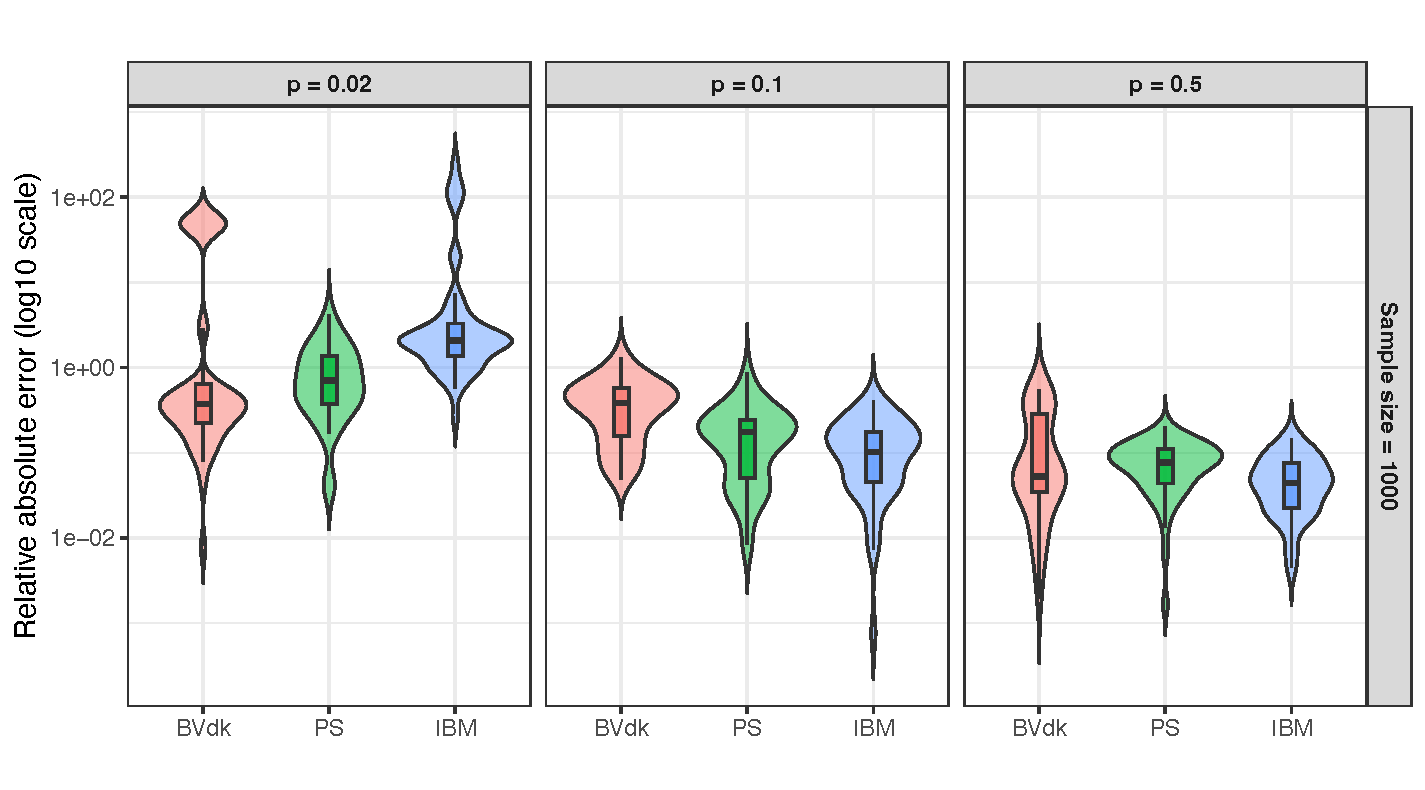
\includegraphics[width=0.49\linewidth]{small_p} 
\includegraphics[width=0.49\linewidth]{overlap} 

}

\caption{Violin plots of estimation errors of $p$: relative absolute error in the case of low proportion of the unknown component (left panel), absolute error in the case of component overlap (right panel).}\label{fig:FigureOverlap-latex}
\end{figure}

As expected, increasing overlap significantly degrades estimation quality for all methods. In the weak overlap case, \emph{IBM} and \emph{PS} yield comparable and reliable results, with standard deviations of 0.02, while \emph{BVdk} shows higher variability (SD = 0.24), likely due to the limited sample size. Under strong overlap, all estimators deteriorate, but \emph{PS} remains the most stable (SD = 0.04 versus 0.22 for \emph{BVdk} and 0.06 for \emph{IBM}). In the huge overlap case, both \emph{BVdk} and \emph{IBM} become essentially unreliable --- \emph{BVdk} systematically hits the boundary at 0.99, and \emph{IBM} produces estimates well above 1 --- while \emph{PS}, although biased towards low values (median 0.04), at least remains bounded and avoids catastrophic failures. These results are summarised in Table \ref{tab:smallp-overlap-latex}. Overall, in cases of heavy overlap, no estimator can be fully trusted, and the practitioner should be aware that identifiability may be compromised.

\subsection{Misspecification of the known component distribution}\label{misspecification-of-the-known-component-distribution}

We finally investigate the robustness of the estimators when the known component \(g\) is incorrectly specified. We simulate a two-component Gaussian mixture with unknown component \(\mathcal{N}(0,1)\) and true known component \(\mathcal{N}(2,0.5)\). The model is then fitted assuming the known component is \(\mathcal{N}(\mu,0.5)\) with \(\mu \in \{-2,1,1.9,2\}\), spanning from strong misspecification to a well-specified model. Figure \ref{fig:FigureMispec-latex} displays the absolute errors \(|\hat{p}-p|\) for each configuration, and Table \ref{tab:mispecification-latex} reports the associated descriptive statistics.

The impact of misspecification is severe and monotone: the further \(\mu\) is from the true value 2, the larger the estimation errors, regardless of the method. In the well-specified case (\(\mu = 2\)), all three estimators perform well, with \emph{PS} and \emph{IBM} showing the smallest standard deviations (0.026 each). As misspecification increases, performance degrades sharply. Under moderate misspecification (\(\mu = 1\)), \emph{IBM} already produces estimates far above 1 (mean 2.490, max 4.895), making it completely unreliable. \emph{BVdk} also suffers, frequently hitting boundary values. \emph{PS} degrades more gracefully, with estimates remaining in a plausible range (mean 0.686, SD 0.020), though still biased. Under strong misspecification (\(\mu = -2\)), all estimators fail: \emph{IBM} systematically saturates at 5.0, BVdk concentrates near the upper boundary, and even \emph{PS} yields estimates around 0.92 with negligible variance -- a sign that it has converged to a wrong fixed point. Among all edge cases considered, misspecification of the known component appears to be the most damaging scenario, underscoring the importance of a careful preliminary specification of \(g\) before applying any of the estimation procedures.

\begin{figure}

{\centering 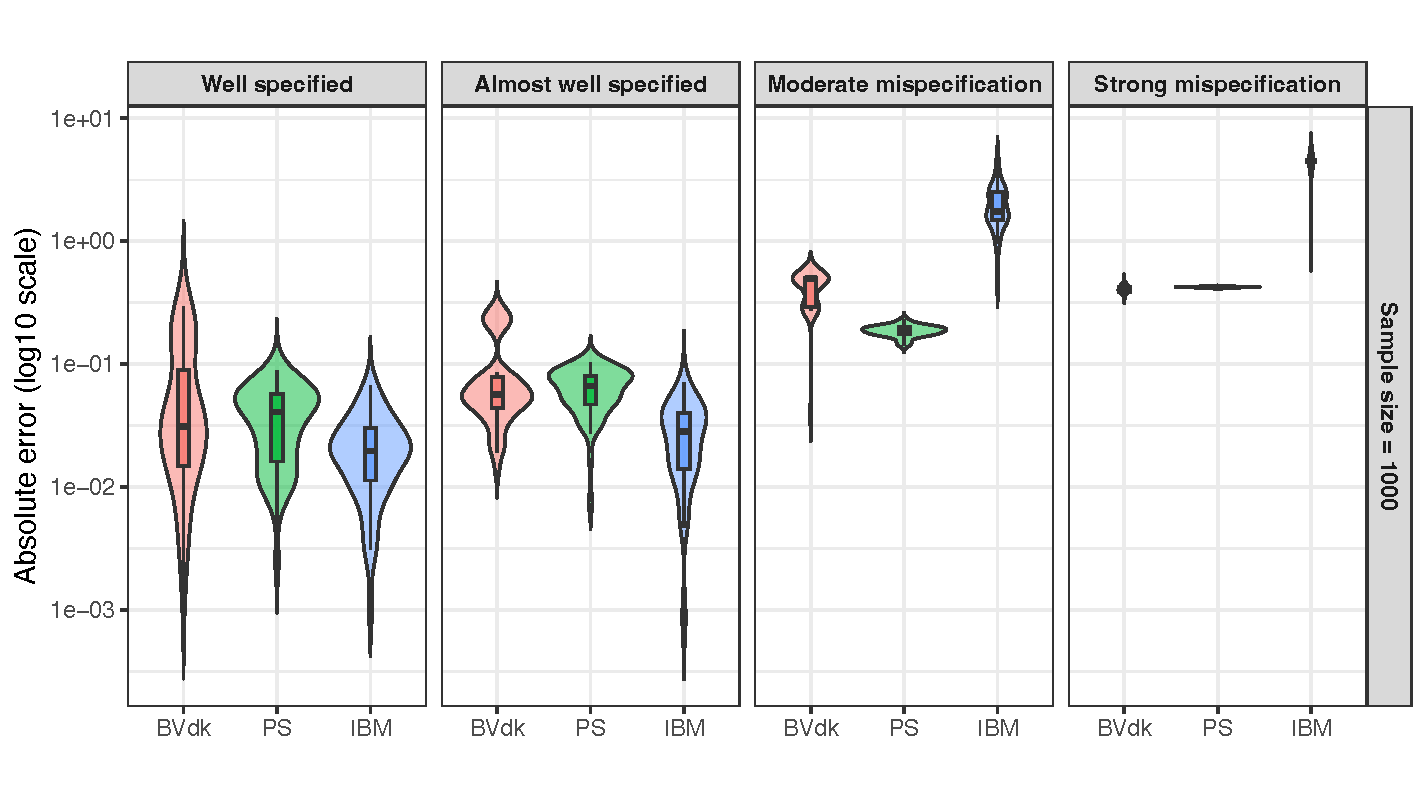
\includegraphics[width=0.55\linewidth,height=0.17\textheight]{mispec} 

}

\caption{Violin plots of the absolute error for the estimation of $p$ for various mispecifications.}\label{fig:FigureMispec-latex}
\end{figure}

\begin{table}[!h]
\centering
\caption{\label{tab:mispecification-latex}Effect of model misspecification on estimation error related to the proportion $p$, for the three estimators.}
\centering
\resizebox{\ifdim\width>\linewidth\linewidth\else\width\fi}{!}{
\fontsize{9}{11}\selectfont
\begin{tabular}[t]{ccccccccccccc}
\toprule
\multicolumn{1}{c}{ } & \multicolumn{3}{c}{Well specified} & \multicolumn{3}{c}{Almost well specified} & \multicolumn{3}{c}{Moderate misspecification} & \multicolumn{3}{c}{Strong misspecification} \\
\cmidrule(l{3pt}r{3pt}){2-4} \cmidrule(l{3pt}r{3pt}){5-7} \cmidrule(l{3pt}r{3pt}){8-10} \cmidrule(l{3pt}r{3pt}){11-13}
  & BVdk & PS & IBM & BVdk & PS & IBM & BVdk & PS & IBM & BVdk & PS & IBM\\
\midrule
Min. & 0.45 & 0.41 & 0.45 & 0.41 & 0.40 & 0.43 & 0.20 & 0.64 & 0.97 & 0.84 & 0.91 & 1.46\\
Q1 & 0.50 & 0.44 & 0.48 & 0.44 & 0.42 & 0.46 & 0.22 & 0.67 & 1.99 & 0.89 & 0.92 & 5.00\\
Med. & 0.53 & 0.46 & 0.50 & 0.45 & 0.43 & 0.47 & 0.99 & 0.69 & 2.24 & 0.90 & 0.92 & 5.00\\
Mean & 0.56 & 0.46 & 0.50 & 0.50 & 0.44 & 0.48 & 0.74 & 0.69 & 2.49 & 0.91 & 0.92 & 4.66\\
Q3 & 0.59 & 0.49 & 0.52 & 0.48 & 0.45 & 0.49 & 0.99 & 0.70 & 3.00 & 0.93 & 0.93 & 5.00\\
Max & 0.80 & 0.52 & 0.57 & 0.78 & 0.49 & 0.52 & 0.99 & 0.73 & 4.90 & 0.99 & 0.93 & 5.00\\
SD & 0.09 & 0.03 & 0.03 & 0.11 & 0.02 & 0.02 & 0.37 & 0.02 & 0.81 & 0.03 & 0.01 & 1.01\\
\bottomrule
\end{tabular}}
\end{table}

\section{Acknowledgments}\label{acknowledgments}

We thank the users of the package for their constructive comments and reported bugs. The package is more and more downloaded, shared and used. This work was conducted within the Research Chair DIALog under the aegis of the Risk Foundation, an initiative by CNP Assurances. D. Pommeret, Y. Salhi and P. Vandekerkhove would also like to acknowledge the support received from the Research Chair ACTIONS under the aegis of the Risk Foundation, an initiative by BNP Paribas Cardif and the French Institute of Actuaries.

\bibliography{milhaud-pommeret-salhi-vandekerkhove.bib}

\address{%
Xavier Milhaud\\
Aix-Marseille University\\%
Department of Statistics\\ 3, Pl. Victor Hugo, 13331, Marseille, France\\
%
\url{https://www.xaviermilhaud.fr/en}\\%
\textit{ORCiD: \href{https://orcid.org/0000-0002-3962-9434}{0000-0002-3962-9434}}\\%
\href{mailto:xavier.milhaud@univ-amu.fr}{\nolinkurl{xavier.milhaud@univ-amu.fr}}%
}

\address{%
Denys Pommeret\\
Aix-Marseille University\\%
Department of Statistics\\ 3, Pl. Victor Hugo, 13331, Marseille, France\\
%
\url{https://www.i2m.univ-amu.fr/perso/denys.pommeret/start}\\%
%
\href{mailto:denys.pommeret@univ-amu.fr}{\nolinkurl{denys.pommeret@univ-amu.fr}}%
}

\address{%
Yahia Salhi\\
University Lyon 1\\%
Institut de Science Financière et d'Assurances\\ 50, Avenue Tony Garnier, 69007, Lyon, France\\
%
\url{http://salhi.yahia.free.fr}\\%
%
\href{mailto:yahia.salhi@univ-lyon1.fr}{\nolinkurl{yahia.salhi@univ-lyon1.fr}}%
}

\address{%
Pierre Vandekerkhove\\
University Gustave Eiffel\\%
5, Boulevard Descartes, 77420 Champs-sur-Marne, France\\
%
\url{https://perso.math.u-pem.fr/vandekerkhove.pierre/}\\%
%
\href{mailto:pierre.vandekerkhove@univ-eiffel.fr}{\nolinkurl{pierre.vandekerkhove@univ-eiffel.fr}}%
}
